\chapter{Introduction to Cosmology}\label{introduction}
\justifying
\section{The Center of the Universe}

One of the foundations of modern cosmology is the Cosmological Principle. If we view it over a large scale, the universe is independent of the position i.e. \emph{homogeneous}, and independent of direction i.e. $isotropic$ to a first approximation.
The spacetime geometry that is consistent with the universe being homogeneous and isotropic is given by the Friedmann-Robertson-Walker Metric(FRW) metric.
\begin{align}
     ds^2= -c^2dt^2 + a(t)^2\left(\frac{dr^2}{1-k r^2}+ r^2d\theta^2 +r^2\sin^2\theta d\phi^2\right ),\label{eq:1.1}
\end{align}\\
where $k = 0$, $k = +1$ and 
$k = -1$ for flat, positively curved and negatively curved space-like $3$-hypersurfaces, respectively. Whereas, $a(t)$ is the scale factor that incorporates the expansion of the universe.\footnote{The line element in \eqref{eq:1.1} has a scaling symmetry i.e $a \rightarrow \lambda a$, $r \rightarrow \frac{r}{\lambda}$, $k \rightarrow \lambda^{2} k$. We can use this freedom to set the scale factor to unity today i.e $a_{0} =1$} For ease of notation, we will restrict most of our discussion to the case $k = 0$.
\hspace{0.5cm}\\
We can write the FRW metric in the flat space i.e. taking the form of the Minkowski metric with the scale factor.

\begin{align}
    d{s^2} = -\ d{t^2} + a^2(t) \ d{\sigma^2}\label{eq:1.2}
\end{align}\\
where 
\begin{align}
     d{\sigma^2} = \gamma_{ij} \ d{x^{i}} \ d{x^{j}}\label{eq:1.3}
\end{align}\\
with 
\begin{align}
    \gamma_{ij}= \delta_{ij} + k\frac{x_{i}x_{j}}{1-k(x_k x^k)}\label{eq:1.4}
\end{align}\\
\hspace{0.5cm}We can notice that by using the polar coordinates we can get to equation Eq. \eqref{eq:1.1}. The polar coordinate used in the equation \eqref{eq:1.1} refers to the observer comoving with the expansion of the universe. We get the physical distance by multiplying the comoving distance with the scale factor.\\
We can redefine the radial coordinate as  
\begin{align}
    d\chi = \frac{dr}{\sqrt{1-k r^2}}\label{eq:1.5}
\end{align}\\
such that,
\begin{align}
   ds^2= -dt^2 + a(t)^2\left[{d\chi^2}+ f(\chi)^2(d\theta^2 +\sin^2\theta d\phi^2)\right ]\label{eq:1.6}
\end{align}\\
where,
\begin{align}
    f(\chi) = \begin{cases}
        sinh\chi,& k=-1\\
        \chi,& k=0\\
        sin\chi,& k=+1
    \end{cases}
\end{align}\\
This form of metric is particularly convenient for studying the propagation of light. Light travels along the null geodesic $ds^2=0$ so to make the propagation of light in FRW similar to the Minkowski space we introduce conformal time,
\begin{align}
    d\tau = \frac{dt}{a(t)},\label{eq:1.8}
\end{align}\\
Substituting it in \eqref{eq:1.6} we get 
\begin{align}
    ds^2= -a(\tau)^2\left[d\tau^2 - \left({d\chi^2}+ f(\chi)^2(d\theta^2 +sin^2\theta d\phi^2)\right)\right ]\label{eq:1.9}
\end{align}

%%%%%%%%%%%%%%%%%%%%%%%%%%%%%Freidmann Equation}%%%%%%%%%%%%%%%%%%%%%%%%%%%%%%%%%%%%%%%%%%%%%    
\section{Friedmann Equation}
\hspace{0.5cm}The dynamics of the way the universe evolves are determined by the Einstein equation.
\begin{align}
    G_{\mu \nu } = R_{\mu \nu } - \frac{1}{2} g_{\mu \nu } R = 8 \pi G T_{\mu \nu }\label{eq:1.10}
\end{align}\\
This relates to the Einstein tensor $G_{\mu \nu }$ which is a measure of the “space-time curvature” of the FRW
universe to the stress-energy tensor where $T_{\mu \nu }$ describes the “matter content” of the universe.\\

\subsection{Space-time Curvature}
\hspace{0.5cm}Let us compute the Einstein tensor on the l.h.s. of the Einstein equation $G_{\mu \nu } = R_{\mu \nu } - \frac{1}{2} g_{\mu \nu } R$ \\ 
The Ricci tensor is given by :
\begin{align}
        R_{\mu \nu } = \Gamma^{\alpha }_{\mu \nu , \alpha } 
        - \Gamma^{\alpha }_{\mu \alpha , \nu }
        + \Gamma^{\beta }_{\mu \nu } \Gamma^{\alpha }_{\alpha \beta } 
        - \Gamma^{\beta}_{\mu \alpha } \Gamma^{\alpha }_{\nu \beta }
\end{align}
Let us see the Christoffel symbols for the FRW metric:
%\begin{claim}
\begin{subequations}
    \begin{align}
        %\begin{gather}
            \Gamma^{0}_{\mu \nu } &= \left[\begin{array}{cccc}
            0 & 0 & 0 & 0 \\ 
            0 & \frac{\dot{a}a}{1-kr^2} & 0 & 0 \\ 
            0 & 0 & r^2a \dot{a} & 0 \\ 
            0 & 0 & 0 & r^2 a \dot{a} \sin^2\theta 
            \end{array}\right]\label{eq:1.12a} \\
            \Gamma^{1}_{\mu \nu } &= \left[\begin{array}{cccc}
            0 & \dot{a} / a & 0 & 0 \\ 
            \dot{a} / a & \frac{kr}{(1-kr^2)} & 0 & 0 \\ 
            0 & 0 & (kr^2-1)r & 0 \\ 
            0 & 0 & 0 & (kr^2-1)r \sin^2\theta 
            \end{array}\right] \label{eq:1.12b}\\ 
            \Gamma^{2}_{\mu \nu } &= \left[\begin{array}{cccc}
            0 & 0 & \dot{a} / a & 0 \\ 
            0 & 0 & 1 / r & 0 \\ 
            \dot{a} / a & 1/r & 0 & 0 \\ 
            0 & 0 & 0 & - \sin \theta \cos \theta 
            \end{array}\right]\label{eq:1.12c} \\ 
            \Gamma^{3}_{\mu \nu } &= \left[\begin{array}{cccc}
            0 & 0 & 0 & \dot{a} / a \\ 
            0 & 0 & 0 & 1/r \\ 
            0 & 0 & 0 & \cos \theta  /\sin \theta  \\ 
            \dot{a} /a  & 1/r & \cos \theta  /\sin \theta  & 0
            \end{array}\right] \label{eq:1.12d}\\ 
        %\end{gather}
    \end{align}
\end{subequations}
%\end{claim}
   

Here we used simplifications that the FRW metric is diagonal, and it does not depend on \(\varphi \).\\

The components of the Ricci tensor are: 
    
\begin{subequations}
    \begin{align}
        R_{00} & = - 3 \partial_{t} (\frac{\dot{a}}{a})  - 3 (\frac{\dot{a}}{a})^2\\
        & = -3 \left(\frac{\ddot{a}}{a} - (\frac{\dot{a}}{a})^2 + (\frac{\dot{a}}{a})^2\right)\\ 
        & = - 3 \frac{\ddot{a}}{a}
    \end{align}
\end{subequations}
    


    
\begin{subequations}
    \begin{align}
        \begin{split}
            R_{11} &= \partial_{t} (\frac{\dot{a} a}{1 - kr^2} )
            + \partial_{r} (\frac{kr}{1 - kr^2})
            - \partial_{r} (\frac{kr}{1 - kr^2})
            - 2 \partial_{r} (\frac{1}{r}) \\
            &\phantom{=}\ 
            + \frac{\dot{a} a}{1 - kr^2} 3 \frac{\dot{a}}{a}
            + \frac{kr}{1-kr^2} (\frac{kr }{1 - kr^2} + \frac{2}{r}) \\
            &\phantom{=}\ 
            - 2 \frac{\dot{a}}{a} \frac{\dot{a} a}{1 - kr^2}
            - (\frac{kr}{1 - kr^2})^2 
            - 2 (\frac{1}{r})^2
        \end{split}  \\
        &= \frac{\ddot{a} a + \dot{a}^2}{1 - kr^2} 
        + 3 \frac{\dot{a}^2}{1 - kr^2}
        + 2 \frac{k}{1 - kr^2}
        - 2 \frac{\dot{a}^2}{1 - kr^2}  \\
        &= \frac{\ddot{a} a + 2 \dot{a}^2 + 2 k}{1 - kr^2}
    \end{align}
\end{subequations}
    
\begin{subequations}
    \begin{align}
        \begin{split}
            R_{22} &= 
            r^2 \partial_{t} (a \dot{a})
            + \partial_{r} ((kr^2-1)r)
            - \partial_{\theta } (\frac{\cos \theta }{\sin \theta }) \\
            &\phantom{=}\ 
            +3 \Gamma^{t}_{\theta \theta } \Gamma^{\theta }_{t \theta } + \Gamma^{r}_{\theta \theta } (\Gamma^{r}_{r r } + 2 \Gamma^{\theta }_{r \theta })
            -2 (\Gamma^{t}_{\theta \theta } \Gamma^{\theta }_{t \theta } + \Gamma^{r}_{\theta \theta } \Gamma^{\theta }_{\theta r}) - \frac{\cos^2 \theta}{\sin^2\theta }
        \end{split}  \\
        &= r^2 (\ddot{a} a + \dot{a}^2)
        + 3kr^2 - 1 + \frac{1}{\sin^2\theta} 
        +  r^2 \dot{a}^2
        - kr^2
        - \frac{\cos^2\theta }{\sin^2\theta }  \\
        &= r^2 (\ddot{a} a + 2\dot{a}^2 + 2k)
    \end{align} 
\end{subequations}

\begin{subequations}
    \begin{align}
        R_{33} &= \partial_{\alpha } \Gamma^{\alpha }_{\varphi \varphi } - \partial_{\varphi } \Gamma^{\alpha }_{\alpha \varphi } + \Gamma^{\alpha }_{\varphi \varphi } \Gamma^{\beta }_{\alpha \beta } - \Gamma^{\beta }_{\varphi \alpha } \Gamma^{\alpha }_{\varphi \beta }  \\
        &= r^2 \sin^2\theta (\ddot{a} a + 2 \dot{a}^2 + 2k) 
    \end{align}
\end{subequations}


The Ricci scalar then comes out to be 

\begin{subequations}
    \begin{align}
        \begin{split}
            R = g^{\mu \nu } R_{\mu \nu } 
            &= 3 \frac{\ddot{a}}{a} 
            + \frac{1-kr^2}{a^2} \frac{\ddot{a}
             a + 2 \dot{a}^2 + 2k}{1 - kr^2} \\
             &\phantom{=}\ 
            + \frac{1}{a^2r^2} r^2 (\ddot{a} a + 2 \dot{a}^2 + 2k)
            + \frac{1}{a^2r^2 \sin^2\theta }
            r^2 \sin^2\theta  (\ddot{a} a + 2 \dot{a}^2 + 2k) 
        \end{split}
        \\
        &= 3 \frac{\ddot{a}}{a} + 3 \frac{\ddot{a}a + 2 \dot{a}^2 + 2k}{a^2}
        \\
        &= 6 \left[\frac{\ddot{a}}{a} + (\frac{\dot{a}}{a}) + \frac{k}{a^2}\right]
        \,.
    \end{align}
\end{subequations}

We find that the non-zero components of the Einstein tensor $G^{\mu}_{\nu} = g^{\mu \lambda}G_{\lambda \nu }$
\begin{subequations}
    \begin{align}
        G^{0}_{0} = 3 \left[\left(\frac{\dot{a}}{a}^2\right) + \frac{k}{a^2}\right]\label{eq:1.18a}
    \end{align}
    \begin{align}
        G^{i}_{j} =  \left[2\frac{\ddot{a}}{a} + \left(\frac{\dot{a}}{a}^2\right) + \frac{k}{a^2}\right]\delta^{i}_{j}\label{eq:1.18b}
    \end{align}
\end{subequations}
\hspace{0.5cm}\\

*\subsection{Stress-energy Tensor}
\hspace{0.5cm}For the universe to be isotropic and homogeneous it is forced to be a perfect fluid. Perfect fluids have a stress-energy tensor like :
\begin{align}
    T^{\mu \nu } =  (\rho + P) u^{\mu } u^{\nu } + P g^{\mu \nu }\label{eq:1.19}
\end{align}\\

where $u^{\mu }$ is the 4-velocity of the fluid element. It is diagonal in the $\emph{comoving frame}$, in which $u^{\mu } = (1, \vec{0})$.\\
\hspace{0.5cm}If we take the covariant divergence of the Einstein tensor \(G_{\mu \nu }\) we get zero; so the stress-energy tensor must also have \(\nabla_{\mu} T^{\mu \nu }=0\). 
One key emphasis here is that the covariant derivative of the stress-energy tensor is not a conservation equation unlike in special relativity where the equation  \(\partial_{\mu}  T^{\mu \nu }\) describes a conservation equation, a local one.\\ 
\hspace{0.5cm}In GR we get a conserved quantity if the metric doesn't depend on some coordinate ($\equiv$ something constant). 
We denote Killing Vectors, a vector oriented in the direction of symmetry. But in cosmology, we do not have symmetry with respect to time translation, so there is no time-like Killing vector \(\xi_{\mu }\) such that \(\xi_{\nu } \nabla_{\mu } T^{\mu \nu }\) represents the conservation of energy.\\
This equation, \(\nabla_{\mu } T^{\mu \nu }\) follows from the fact that our fluid follows its equations of motion. 
Let us explore the meaning of these equations. If, in the equation \( \nabla_{\mu } T^{\mu}_{0} = 0\),  we find 
\begin{subequations}
    \begin{align}
        \nabla_{\mu } T^{\mu}_{0} 
        &= \partial_{\mu } T^{\mu }_{0} + \Gamma^{\mu }_{\mu \lambda } T^{\lambda }_{0} - \Gamma^{\lambda }_{\mu 0} T^{\mu }_{\lambda }
        = 0 
    \end{align}
\begin{quote}
        the term $T^{i}_{0}$ vanishes by isotropy. So we get,
\end{quote}
    \begin{align}
        \partial_{t} \rho + \Gamma^{\mu }_{\mu 0} \rho - \Gamma^{\lambda }_{\mu 0} T^{\mu }_{\lambda } = 0 
    \end{align}
\begin{quote}
        From \eqref{eq:1.12b},\eqref{eq:1.12c},\eqref{eq:1.12d} we see that $\Gamma^{\lambda }_{\mu 0}$ vanishes
        unless $\lambda$ and $\mu$ are spatial indices equal to each other, in which case it is $\frac{\dot{a}}{a}$.The above equation therefore reads :
\end{quote}
    \begin{align}
        \dot{\rho} + 3 \frac{\dot{a}}{a}(\rho + P) = 0 \label{eq:1.20c}
    \end{align}
\end{subequations}
To find the other two Friedmann equations we compare the time-time equation and the space-space equation of the Einstein equations to the stress-energy tensor i.e comparing \eqref{eq:1.19} to \eqref{eq:1.18a} and \eqref{eq:1.18b} respectively
To relate the sources of matter to the evolution of the scale factor in the FRW metric \eqref{eq:1.9}, 
\begin{subequations}
    \begin{align}
        \frac{\ddot{a}}{a} &= - \frac{4 \pi G}{ 3} (\rho + 3 P) \label{eq:1.21a}  \\
        \left(\frac{\dot{a}}{a}\right)^2 &= \frac{8 \pi G}{3} \rho - \frac{k}{a^2} \label{eq:1.21b}
    \end{align}
\end{subequations}\\
The space-space equation is not a dynamical equation, since it contains no second-time derivatives: it is a \emph{constraint} on the evolution of the system. 
However, the three Friedmann equations are not independent: the time-time one can be found from \eqref{eq:1.21a} and \eqref{eq:1.20c}.\\
We define $\left(\frac{\dot{a}}{a}\right) \equiv H $, the Hubble parameter which is the measure of the expansion rate of the universe, measured in $Km.s^{-1}.Mpc^{-1}$.\\ 
\hspace{0.5cm}The above equations \eqref{eq:1.20c},\eqref{eq:1.21a},\eqref{eq:1.21b} describe how the universe expands and lay the groundwork for all further discussion of cosmology.
We can solve the Friedmann equations by an equation of state that relates $\rho$ to $P$. 
\begin{align}
    w = \frac{P}{\rho} . 
\end{align}
Plugging it in the continuity equation \eqref{eq:1.20c} we get:
\begin{align}
    \frac{ \log \rho}{ \log a} = {-3(1 + w)} \implies \rho \propto a^{-3(1 + w)}\label{eq:1.23} 
\end{align}\\

\begin{align}
    \rho(a) \propto 
    \begin{cases}
        a^{-4} ,& \text{radiation: }  w =\frac{1}{3}\\
        a^{-3},              & \text{matter: }  w = 0\\
        \text{constant},              & \text{dark energy: }  w = -1\\
    \end{cases}\label{eq:1.24}
\end{align}
It makes intuitive sense that the energy density of relativistic particles decreases as the universe expands, not only because the average number of particles per unit volume decreases ($V \propto a^3$), as it does for non-relativistic matter, but also because of the relativistic Doppler shift, which increases the negative power of the scaling factor by one. 
In contrast, dark energy has a constant energy density. 
Assuming the universe is composed of three different kinds of fluids, radiation, matter, and dark energy, then each has successively dominated the energy budget of the universe and shaped its history at various epochs.\\
Now, combining \eqref{eq:1.23} with the first Friedmann equation \eqref{eq:1.12b} we get the time dependence of the scale factor.
\begin{align}
    a(t) \propto 
    \begin{cases}
        t^{\frac{2}{3(1+w)}} ,& \text{if,}  w\neq -1\\
        e^{Ht},               & \text{if,}  w = -1\\
    \end{cases}\label{eq:1.25}
\end{align}\\
We can observe that for $w = 0$, which corresponds to a Universe dominated by non-relativistic matter, we get $a(t) \propto  t^{2/3}$. 
Now, for $w = 1/3$, which corresponds to relativistic particles (radiation), we get $a(t) \propto  t^{1/2}$. 
The last and very relevant case is $w = -1$, corresponding to a fluid exerting negative pressure, which leads to the second solution in Eq. \eqref{eq:1.25}, i.e. an exponential expansion describes the Dark Energy.



%%%%%%%%%%%%%%%%%% The Cosmological Constant  %%%%%%%%%%%%%%%%%%%%%%%%%%%%%%%%%%%%%%%%%%%%%%%%%

\section{The Cosmological Constant}
\hspace{0.5cm}When Einstein developed his theory of general relativity, the prevailing belief was that the Universe was static. However, this contradicted the Friedmann equations, which showed that a Universe
evolving according to them could not be static unless the acceleration  $\vec{a}$ was zero. namely
\begin{align}
   \rho=-3 P \label{1.26}
\end{align}
Since a fluid with such property did not seem to be physically reasonable, Einstein modified Eq. \eqref{eq:1.10} by introducing the cosmological constant term $\Lambda$ to counterbalance the gravitational attraction
\begin{align}
    R_{\mu \nu}-\frac{1}{2} g_{\mu \nu} R=8 \pi G T_{\mu \nu}-\Lambda g_{\mu \nu},\label{1.27}
\end{align}
 in such a way that it does not change the covariant character of the equations. It can be shown that for an appropriate choice of $\Lambda$, one indeed obtains a static cosmological model.
In order to recover a form similar to the Eq. \eqref{eq:1.10}, we rewrite the stress-energy tensor in a more compact way

\begin{align}
    \bar{T}_{\mu \nu} & =T_{\mu \nu}-\frac{\Lambda}{8 \pi G} g_{\mu \nu} \\ & =(\bar{P}+\bar{\rho}) u_\mu u_\nu+\bar{P} g_{\mu \nu}, \label{1.29}
\end{align}

so that
\begin{align}
    R_{\mu \nu}-\frac{1}{2} g_{\mu \nu} R=8 \pi G \bar{T}_{\mu \nu}\label{1.30}
\end{align}


In Eq. \eqref{1.29}, the effective pressure $\bar{P}$ and the effective density $\bar{\rho}$ are related to the corresponding quantities for a perfect fluid by
\begin{align}
    \bar{P}=P-\frac{\Lambda}{8 \pi G}, \quad \bar{\rho}=\rho+\frac{\Lambda}{8 \pi G}\label{1.31}
\end{align}

Although after the discovery of the expansion of the Universe in the late 1920s, there was no need for a term that made the Universe static, the cosmological constant remained a subject of great interest and it is today the simplest possible explanation for the observed accelerated expansion of the Universe. The standard model of cosmology that incorporates the effects of the cosmological constant is the $\Lambda$CDM model.

One cosmological model that involves the cosmological constant is the de Sitter Universe. In this model, the Universe is dominated by a positive cosmological constant, which suppresses all other matter contributions, making the Universe empty ($\rho=0$),($P = 0$) and flat ($k=0$). Under these conditions, the effective pressure and density are related to the cosmological constant through equation \eqref{1.31} we get,
\begin{align}
   \bar{P}=-\bar{\rho}=-\frac{\Lambda}{8 \pi G}, \label{1.32}
\end{align}

which, if replaced in Eq. \eqref{eq:1.21b} gives
\begin{align}
    \frac{\dot{a}^2}{a^2}=H^2=\frac{\Lambda}{3},\label{1.33}
\end{align}

corresponding to a Hubble parameter constant in time.The solution to
this equation is an exponential expansion, where the scale factor increases as a function of time
\begin{align}
    a \propto \exp \left(\sqrt{\frac{\Lambda}{3}} t\right),\label{1.34}
\end{align}


This exponential expansion means that test particles move away from
each other due to the repulsive gravitational effect of the positive cosmological constant.



%%%%%%%%%%%%%%%%%%%%%%%%%%%%%%%%%%%%%%%Cosmic Distances%%%%%%%%%%%%%%%%%%%%%%%%%%%%%%%%%%%%%%%%%%%%%%
\section{Cosmic Distances} 
 The Universe is observed to be expanding, and the scale factor $a(t)$ is increasing with time. This expansion also affects the photons that were emitted a long time ago far away and reach us today, which become redshifted due to the stretching of space. Therefore, it is convenient to define a quantity that describes the distance - and time - of a patch of the Universe we are observing based on this physical effect. For that, we define the redshift $z$ as
\begin{align}
    z+1 = \frac{a(t0)}{a(t)}
\end{align}
where $t$ is the time when the signal was emitted and $t_0$ is today. The scale factor is defined up to a multiplicative constant, and it's usually assumed $a(t_0) = 1$, so $z + 1 = a(t)^{-1}$.
As we know, the causal connection of points in space-time is determined by whether they are inside or outside each other's lightcone. Lightcones are the solutions to the equation
\begin{align}
ds^2 = 0,
\end{align}
where $ds^2$ is the space-time interval between two events. In other words, the lightcone of an event consists of all the events that could potentially receive a signal from the first event, assuming the signal travels at or below the speed of light.\footnote{In this section we use c = 1} Any event inside the past lightcone of another event can be causally influenced by it, while any event outside the future lightcone cannot be influenced by it.
With $ds^2$ a suitable metric, in our case the FRW metric Eq. \eqref{eq:1.6}, assuming a homogeneous and isotropic Universe and taking $d\Omega=0$,the comoving particle horizon is then, 
\begin{align}
    r_p(t) \equiv \chi(t) = \int_0^t \frac{ dt'}{a(t')} =  \int_0^a d\ln{a}\left(\frac{1}{aH}\right) = \tau \label{eq:1.28}
\end{align}

where in the last equality we exploited the relation we found earlier for the conformal time  Eq. \eqref{eq:1.8}\footnote{The main benefit of working with conformal time: light rays correspond to straight lines at $45 \degree$ angles in the $\chi - \tau$ coordinates. If instead, we had used physical time t, then we would find the light cones for curved space-times would be curved.}.

The comoving horizon is therefore the logarithmic integral of the comoving Hubble radius $\frac{1}{aH}$, which we will define below. The related physical particle horizon is
\begin{align}
    d_p(t) = a(t) r_p(t) = a(t) \int_0^t \frac{ dt'}{a(t')} \label{eq:1.29}
\end{align}

due to the scale factor in the denominator and the fact that $a(t) \rightarrow 0$ as $t$ goes to 0, the particle horizon could become infinite, meaning that an observer would be in causal connection with the whole Universe. Using Eq. \eqref{eq:1.25}, we can find an approximate expression for $d_p(t)$ for $w > -1/3$, or else we can notice that the integral diverges. Using the Hubble parameter in FRW model which is 
\begin{align}
    H = \frac{2}{3(1+w)t}
\end{align}
 With $w = 0$, a spatially flat matter-dominated universe, $H = 2/3t$ and $a \propto  t^ {\frac{2}{3}}$. With $w = 1/3$, a spatially flat radiation-dominated universe, we have $H = 1/2t$ and $a \propto  t^ {\frac{2}{3}}$.
we can write Eq. \eqref{eq:1.29} as

\begin{align}
d_p(t) \simeq \frac{3(1+w)}{1+3w}t = \frac{2}{1+3w}\frac{1}{H}
\end{align}

We take into note that $w > -1/3$ implies $\ddot{a} < 0$, a decelerating expansion which means
we have a finite particle horizon only in the case of a primordial universe characterized by a decelerating universe.
Now, let us look into the Hubble time and the comoving Hubble radii.

\begin{align}
    t_{H} = \frac{a}{\dot{a}} = \frac{1}{H} \\                  
    r_{H} = \frac{R_{H}}{a} = \frac{1}{\dot{a}} = \frac{1}{aH} \footnote{$R_{H} = t_{H}$}  \label{eq:1.33}
\end{align}

The Hubble radius, which is given by $(aH)^{-1}$, represents the distance that particles can travel during one expansion time. It is a measure of whether particles can communicate with each other within a given time frame, based on their comoving separation $\lambda$. In contrast, the particle horizon represents the maximum distance from which particles can reach us within the age of the Universe. Thus, while both the Hubble radius and particle horizon are related to the causal connection of particles, they differ conceptually in that the former measures whether particles can communicate within a given time frame, while the latter measures the maximum distance from which particles can reach us.
\begin{enumerate}
    \item if $\lambda$ \ \textgreater  particle horizon, then the particles could never have communicated.
    \item if $\lambda$ \textgreater  $(aH)^{-1}$ then the particles can't communicate now.
\end{enumerate}



%%%%%%%%%%%%%%%%%%%%%Cosmic Accounting: The Universe's Energy Budget%%%%%%%%%%%%%%%%%%%%%

\section{Cosmic Accounting: The Universe's Energy Budget} \label{section 1.4}
\hspace{0.5cm}As we saw previously in solving the Friedmann equations using the equation of state $w$, the universe is composed of various ingredients, which prompts us to consider their individual contributions to the cosmic energy budget. 
In this section, we explore the cosmic accounting of the universe's energy budget and investigate the different components that make up the cosmic inventory. We follow \cite{Baumann_2022} for the discussion.
Let us look back into Eq.  \eqref{eq:1.21b} and re-write it using the Hubble parameter $H$, we get
\begin{align}
    H^2 = \frac{8 \pi G}{3} \rho - \frac{k}{a^2} \label{eq:1.43}
\end{align}
We will use the subscript '0' to denote the quantities evaluated today, at $t= t_0$. Considering a flat universe$(k = 0)$ the density required for it corresponds to the critical density today denoted by $\rho_c$
\begin{align}
    \rho_{crit,0} =\frac{3H_{0}^{2}}{8\pi G} \label{eq:1.35}
\end{align}
We use critical density to define dimensionless density parameters
\begin{align}
    \Omega_{I,0} \equiv \frac{\rho_{I,0}}{\rho_{crit,0}}\label{eq:1.36}
\end{align}
We can write the Friedmann equation Eq. \eqref{eq:1.43} as
\begin{align}
    H^2(a) = H_{0}^2 \left[\Omega_{r,0}\left(\frac{a_0}{a}\right)^4 + \Omega_{m,0}\left(\frac{a_0}{a}\right)^3 + \Omega_{k,0}\left(\frac{a_0}{a}\right)^2 +\Omega_{\Lambda,0}\right] \label{eq:1.37}
\end{align}
where $I = (r,m,k,\Lambda)$ stands for radiation, matter, curvature, and vacuum energy contribution respectively and we defined a $curvature$ density parameter $ \Omega_{k,0} \equiv \frac{-k}{(a_0H_0)^2}$. From now on we will drop the subscript "0" and just write it as  $\Omega_{r}$ which means the radiation density today. So Eq. \eqref{eq:1.37} becomes
\begin{align}
     \frac{H^2}{H_{0}^2} = [\Omega_{r}a^4 + \Omega_{m}a^3 + \Omega_{k}a^2 +\Omega_{\Lambda}] \label{eq:1.38}
\end{align}
At the current time, the scale factor is $a(t_0) = 1$ and $H =H_0$.Substituting the values in \eqref{eq:1.38} we get
\begin{align}
    \Omega_{total} = \Omega_{r} + \Omega_{m} + \Omega_{k} +\Omega_{\Lambda} = 1 \label{1.39}
\end{align}
so, we can say that the density parameter represents the energy content of the universe. Observations show that the universe is filled with radiation($r$), matter ($m$), and dark energy($\Lambda$).
\begin{align}
    |\Omega_k| \leq 0.01 , \Omega_r = 9.4 \times 10^{-5} , \Omega_m = 0.32 , \Omega_{\Lambda} =0.68 \label{1.40}
\end{align}
As we can see, the curvature only accounts for 1\% of the total energy budget. Curvature's effects were inconsequential earlier(the curvature contribution is only $10^{-2}$).The matter density parameter is further split into Baryons($b$) and DM($c$).\\
\hspace{0.5cm}The predictions of primordial nucleosynthesis, which postulates that the density of protons and neutrons in the early Universe affects the efficiency with which fusion occurs, provide the best current constraints on the baryon density of the universe. Deuterium and other elements found in primordial gas clouds have been studied, and the results suggest that the density parameter of baryonic matter is $\Omega_{b} = 0.05$. 
The majority of the matter density parameter is contained in $non-baryonic$ matter called DM $\Omega_{c} = 0.27$.This 27\% of the universe's energy budget is one of the most enigmatic substances in the universe, which has been an active topic of research.\\
\hspace{0.5cm} Of the radiation contribution majority of it comes in the form of the photons from the cosmic microwave background (CMB) however, experiments such as the \emph{Planck} satellite have found clear evidence for relativistic particles in addition to the known Photons and is compatible with the expected cosmic neutrino contribution\cite{planckcollaboration2019planck2018resultsix}. This will be explored in more detail in Chapter \ref{neutrinos}.
\hspace{0.5cm} 





%%%%%%%%%%%%%%%%%%%%%%%%%%%%%%%%%%%%%%%%%%%%%%%%%%%%%%%%%%%%%%%%%%%%%%%%%%%%%%
%%%%%%%%%%%%%%%%%%%%%%%%%%%%%%%%%%%%%%%%%%%%%%%%%%%%%%%%%%%%%%%%%%%%%%%%%%%%%%%
\section{Thermal History of the Universe} \label{thermal history}

In this section, we outline the thermal history of the standard hot big bang universe as the temperature of the plasma decreased from approximately $10^{11} \, \text{K}$ to $10^{8} \, \text{K}$, following \cite{Weinberg:2008zzc}. During this period, two significant events occurred: neutrinos decoupled from the plasma, and shortly afterwards, electrons and positrons annihilated, leading to the heating of photons relative to neutrinos. Our goal is to understand how these events influenced the evolution of the energy densities of photons and neutrinos.

For massless particles described by the Fermi-Dirac or Bose-Einstein distributions, the energy density is given by

\begin{equation}
    \rho(T)= 
    \begin{cases}
        g \frac{\pi^{2}}{30} T^{4} & \text{Boson} \\
        \frac{7}{8} g \frac{\pi^{2}}{30} T^{4} & \text{Fermion}
    \end{cases}\label{1.50}
\end{equation}

where $g$ counts the number of distinct spin states. The entropy density for massless particles is given by

\begin{equation}
    s(T)=\frac{4 \rho(T)}{3 T}\label{1.51}
\end{equation}

It is convenient to define a quantity $g_{\star}$ which counts the spin states for all particles and antiparticles, with an additional factor $\frac{7}{8}$ for fermions. With this definition, the total energy density and entropy density of the Universe during radiation domination are given by

\begin{align}
    \rho(T) & = g_{\star} \frac{\pi^{2}}{30} T^{4} \\
    s(T) & = \frac{4}{3} g_{\star} \frac{\pi^{2}}{30} T^{3} \label{1.52}
\end{align}

In an expanding universe, the first law of thermodynamics implies that for particles in equilibrium, the comoving entropy density is conserved:

\begin{equation}
    a^{3} s(T)=\text{const} \label{1.53}
\end{equation}

A straightforward consequence of this conservation is that for radiation in free expansion, the temperature evolves inversely with the scale factor:

\begin{equation}
    T \propto \frac{1}{a}\label{1.54}
\end{equation}

Let's now apply this understanding to the early universe.

At a temperature of $10^{11} \, \mathrm{K} (T \sim 10 \, \mathrm{MeV})$, the universe was filled with photons, electrons, positrons, and neutrinos (and antineutrinos) of three species, all in thermal equilibrium with negligible chemical potential.\footnote{There was also a much smaller density of baryons and dark matter, but they are not significant for the discussion above}. As the temperature of the plasma dropped below approximately $10^{10} \, \mathrm{K}$ (around 1 second after the end of inflation), the rate of collisions between neutrinos and electrons/positrons could no longer keep up with the universe's expansion rate. Consequently, neutrinos fell out of equilibrium and began free expansion. Meanwhile, electrons and positrons remained in equilibrium with photons, and their number densities decreased with the falling temperature, effectively vanishing by the time the temperature reached $T \sim 10 \, \mathrm{keV}$.

For simplicity, we will assume that neutrinos decoupled instantaneously before electron-positron annihilation and will later discuss how more detailed calculations might modify the results. Non-zero neutrino masses can be neglected here as long as $m_{\nu} \lesssim 1 \, \mathrm{keV}$, a condition supported by current observational bounds \cite{PLanck20182020}.

From this point forward, we will differentiate the temperature of neutrinos, $T_{\nu}$, from that of photons, $T_{\gamma}$. Before neutrino decoupling, frequent interactions maintained thermal equilibrium between neutrinos and photons, ensuring a common temperature. After the universe became transparent to neutrinos, they retained their relativistic Fermi-Dirac distribution, with a temperature decreasing inversely with the scale factor. In contrast, photons were heated by the annihilation of electrons and positrons.
The conservation of comoving entropy allows us to compute the relative temperatures at later times.
After neutrino decoupling, but before electron-positron annihilation, the thermal plasma contained two spin states of photons, plus two spin states each of electrons and positrons, which means that during this period,

\begin{equation}
    g_{\star}^{\text{before}}=2+\frac{7}{8}(2+2)=\frac{11}{2} \label{1.55}
\end{equation}

After electron-positron annihilation, only the two spin states of photons remained, and so

\begin{equation}
    g_{\star}^{\text{after}}=2 \label{1.56}
\end{equation}

Since $T_{\nu} \propto a^{-1}$ during this period, the comoving entropy conservation can be expressed as

\begin{equation}
    \frac{g_{\star}^{\text{before}} T_{\gamma, \text{before}}^{3}}{T_{\nu, \text{before}}^{3}}=\frac{g_{\star}^{\text{after}} T_{\gamma, \text{after}}^{3}}{T_{\nu, \text{after}}^{3}} \label{1.57}
\end{equation}

Using the fact that $T_{\gamma, \text{before}}=T_{\nu, \text{before}}$, we find 

\begin{equation}
    \frac{T_{\gamma, \text{after}}}{T_{\nu, \text{after}}}=\left(\frac{11}{4}\right)^{1 / 3} \label{1.58}
\end{equation}

We see that in the instantaneous neutrino decoupling limit, the annihilation of electrons and positrons raised the temperature of photons relative to that of neutrinos by a factor of $(11 / 4)^{1 / 3} \simeq 1.40$.

After electron-positron annihilation, assuming three species of light neutrinos and antineutrinos, each with one spin state, the radiation density of the Universe is

\begin{equation}
    \rho_{r}=\frac{\pi^{2}}{30}\left[2 T_{\gamma}^{4}+6 \frac{7}{8} T_{\nu}^{4}\right]=\frac{\pi^{2}}{15}\left[1+3 \frac{7}{8}\left(\frac{4}{11}\right)^{4 / 3}\right] T_{\gamma}^{4} \label{1.59}
\end{equation}

It is conventional to define a quantity $N_{\text{eff}}$ which gives the radiation energy density in terms of the effective number of neutrino species as

\begin{equation}
    \rho_{r}=\frac{\pi^{2} k_{B}^{4}}{15 \hbar^{3} c^{3}}\left[1+\frac{7}{8}\left(\frac{4}{11}\right)^{4 / 3} N_{\mathrm{eff}}\right] T_{\gamma}^{4} \label{1.60}
\end{equation}

where we have restored $k_{B}, c$ and $\hbar$ for completeness. In the instantaneous neutrino decoupling approximation described above, we found $N_{\text{eff}}=3$. In the real Universe, however, the decoupling of neutrinos is not instantaneous, and the residual coupling of neutrinos at the time of electron-positron annihilation increases $N_{\text{eff}}$ by a small amount in the Standard Model.

Unlike photon decoupling at temperature $k_{B} T \sim 0.2 \mathrm{eV}$, active neutrino decoupling at $T \sim 10 \mathrm{MeV}-0.1 \mathrm{MeV}$ takes place over many tens of Hubble times, with the result that we expect distortions in the relic neutrino energy spectra relative to the thermal relativistic Fermi-Dirac distribution. Standard Model Boltzmann neutrino transport calculations show that these distortions change $N_{\text{eff}}$ at the percent level, with the current best estimate predicting $N_{\text{eff}}=3.046$ \cite{Mangano_2005}. In section \ref{neutrinos} we will see how neutrinos leave a detectable imprint on cosmological observations.






%%%%%%%%%%%%%%%%%%%%%%%%%%%%%%%%%The Early Universe%%%%%%%%%%%%%%%%%%%%%%%%%%%%%%%%%%%%%%%%%%

\section{The Early Universe}
\hspace{0.5cm} The shortcoming of FRW cosmology is that it is unable to explain why the universe we observe is homogeneous and isotropic on larger scales without a finely tuned set of initial conditions, and how the initial seed perturbations for structure formation were generated.

In this chapter, we delve into two of the primary problems of the Hot Big Bang model: the horizon problem and the flatness problem. We explore how inflation, an early period of accelerated expansion, can drive the primordial Universe towards homogeneity and isotropy, even if it begins in a more generic initial state, and also how quantum fluctuations that arise during the inflationary period can give rise to the formation of primordial black holes.

\subsection{The Horizon Problem}
\hspace{0.5cm}Previously we introduced Hubble radii ($r_H = (aH)^{-1}$) Eq.\eqref{eq:1.33} and comoving particle horizon $\tau$ \eqref{eq:1.28} as an integral of the comoving Hubble radii. We could observe that for a universe dominated by the fluid equation of state, $w > -1/3 $ the Hubble radius and the comoving particle horizon grow monotonically with time which implies that the comoving scales entering the horizon today have been far outside the horizon at CMB decoupling. However, we find the CMB to be extremely homogeneous. In other words, at the time of the last scattering, the universe was expected to be homogeneous only on small scales since wider scales would not have been causally connected. However, the observation of the nearly homogeneous CMB suggests that the universe was extremely uniform even on larger scales that should have been independent of each other which was surprising.\\
\hspace{0.5cm}To overcome the horizon problem, it's important to consider the causal contact between particles. If a region, denoted by $\lambda$, has a typical size (constant in comoving scales) that is smaller than $(a_{I}H_{I})^{-1}$, then the particles within that region were in causal contact. However, if $\lambda$ becomes larger than $(a_{I}H_{I})^{-1}$ after a sufficient period of inflation, then these particles can no longer communicate. Therefore, before crossing the Hubble radius and becoming causally disconnected, these particles had the opportunity to communicate with each other and reach similar conditions. This implies that everything within the Hubble sphere at the beginning of inflation, which is $(a_{I}H_{I})^{-1}$, was in causal contact.\\
\hspace{0.5cm} We can hence observe that the horizon problem can be resolved if the comoving Hubble radius at the beginning of inflation, $(a_I H_I)^{-1}$, exceeds the radius of the observable universe, $(a_0 H_0)^{-1}$. In this scenario, the entire observable universe would have been contained within the comoving Hubble radius at the onset of inflation.\\
The duration of the inflation to solve the horizon problem is given by the means of e-folds which is defined as,
\begin{align}
    \mathcal{N} = ln \left( \frac{a_E}{a_I} \right)
\end{align} \label{1.2.1}
from the requirement  $(a_I H_I)^{-1} > (a_0 H_0)^{-1}$ we get $\mathcal{N} \approx 60 $
\begin{figure}[ht]
    \centering
    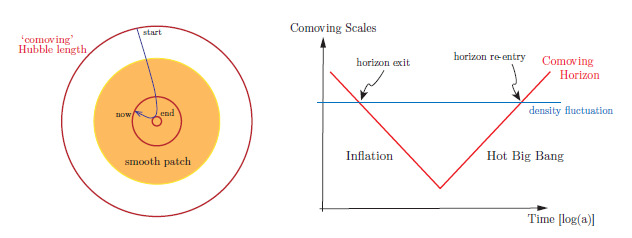
\includegraphics[width=0.7\textwidth]{Images/horizon.png}
    \caption{\emph{Left}: Development of the inflationary universe's $(aH)^{-1}$ comoving Hubble radius. Inflation causes the co-moving Hubble sphere to contract and then expand. Hence, inflation serves as a tool to "zoom in" on a smooth sub-horizon patch. \emph{Right}: Solution of the horizon problem. All scales that are relevant to cosmological observations today were larger than the Hubble radius until $a \sim 10^{-5}$. These scales were, however, smaller than the Hubble radius at sufficiently early eras and were consequently causally related. Similarly, the scales of cosmological interest came back within the Hubble radius in relatively recent times.\cite{baumann2012tasi}}
    \label{fig:1.1} 
\end{figure}

\subsection{The Flatness Problem}
We saw in section \ref{section 1.4} that the current measurements of the density parameters are compatible with a flat universe $\Omega_{total} \simeq 1 $.But the question arises how does $\Omega $ evolve with time?
We can write the Friedmann equation Eq. \eqref{eq:1.43} as 
\begin{align}
    \Omega(t)-1 = \frac{k}{H(t)^{2} a(t)^{2}} \propto  \frac{k}{a^{2-3(1+w)}} = ka^{3w+1} \label{1.2.2}
\end{align}
We observe that for both radiation ($w = 1/3$) and matter ($w = 0$), we see that if $\Omega - 1 \neq 0$ at a certain early time then it will grow as $a^2$ or 
$a^4$ respectively and then the geometry of the present Universe is expected to be curved. So the near-flatness, we observe today requires the value of $\Omega(t)$ to be one. \\
By manipulating the Friedmann equation Eq. \eqref{eq:1.43} we find

\begin{align}
  \Omega ^{-1} (z) -1
  = (\Omega_0 ^{-1} -1)\qty(\frac{T_0 }{T(z)})^{2} \,.
\end{align}

Let us extend this to the Planck epoch because the density at a time $t_P \approx 10^{-43}s$ must have been very close to the critical density. The temperature at that time was $T_P = \num{e32} K $. $T_{0}$ is the temperature today.


If we compute \(T _{\text{Pl}} / T_0 \) we get approximately \num{e32}.

This means that 
\begin{align}
    \Omega^{-1}(z_{\text{Pl}}) - 1 \approx (\Omega_0^{-1} - 1) \num{e-64}\,.
\end{align}
.As a result, the Universe should have needed to be extraordinarily finely tuned in order to imitate the flatness we observe today.

Using the Hubble radius, we can write to examine how the inflationary phase responds to this issue.
\begin{align}
    \Omega(t)-1 = \frac{k}{H(t)^{2} a(t)^{2}} = kr_{H}^2
\end{align}
In standard cosmology, the comoving Hubble radius grows with time,
therefore one expects the quantity $|\Omega(t)-1|$ to grow with time and the geometry of the present Universe to be curved. But,
if the universe undergoes a phase where the Hubble radius shrinks, this would bring $\Omega(t)$ closer to 1. It can be shown that the universe must expand by 60 e-foldings to achieve the flatness we observe today, as in the case of the horizon problem.



\subsection{Dynamics of Inflation}

\hspace{0.5cm}In the previous section, we saw that for inflation to take place we need a phase of accelerated expansion ($\ddot{a} > 0$) where the Hubble radius($r_{H}$) shrinks.\\
We can see from the Friedmann Eq. \eqref{eq:1.21a} that for an accelerated expansion
\begin{align}
    \ddot{a} = -\frac{4 \pi G}{3}(\rho+3P) > 0 \Rightarrow P < \frac{-\rho}{3}\,\label{1.2.6}
\end{align}
which we previously encountered in the de-Sitter model where we found $a(t) \propto exp(\sqrt{\frac{\Lambda}{3}}t)$ and the expansion is driven by cosmological constant $\Lambda$, so we can have a calculated guess that the inflation can't be driven by matter or radiation. In the current interpretation, $\Lambda$ is linked to the quantum fluctuations of the vacuum. The vacuum expectation value of the stress-energy tensor gives the energy generated by these fluctuations.Using Eq. \eqref{eq:1.19} and Eq. \eqref{1.32} we can write
\\
\begin{align}
    \langle T_{\mu\nu} \rangle = -\langle P_{\Lambda} \rangle g_{\mu\nu} = \frac{\Lambda}{8\pi G} g_{\mu\nu} \label{1.2.7}
\end{align}
As a result, in this instance, the stress-energy tensor's vacuum expectation value functions as the cosmological constant that promotes the expansion. This provides an indication of what to anticipate from a theory describing the inflationary mechanism.

\subsubsection{Scalar(Inflaton) Field }





\hspace{0.5cm}To satisfy Eq. \eqref{1.2.6} let us introduce a minimally coupled(i.e not coupled with gravity or any other field ) scalar field \(\varphi\)  with a suitable potential $V(\varphi)$ which is a self-interaction of the field. We can write its Lagrangian as 
\begin{align}
    \mathscr{L}_{\varphi} = -\frac{1}{2} g^{\mu\nu} \partial_{\mu}\varphi\partial_{\nu}\varphi - V(\varphi)\, \label{1.2.8}
\end{align}
The action is in the form of 

\begin{align}
    S = S_{EH} + S_\varphi + S _{\text{matter}}\,\label{1.2.9}
\end{align}

where \(S_{EH}\) is the Einstein-Hilbert action for the metric, \(S_\varphi \) is the action for the field \(\varphi \), while ``matter'' encompasses all the other fields but we can ignore it thanks to the \emph{no-hair cosmic theorem}.

\begin{align}
    S = \frac{1}{16 \pi G} \int \dd[4]{x} \sqrt{-g} R + \int \dd[4]{x} \sqrt{g} \mathscr{L}\varphi [\varphi , g{\mu \nu }],. \label{1.2.10}
\end{align}

We are using the invariant volume element \(\dd[4]{x} \sqrt{-g}\)
representing the physical 4-volume regardless of the coordinates.
Now, we can find the equation of motion for the inflaton field by the Klein-Gordon equation by varying the action with respect to $\varphi$.
\begin{align}
    \square \varphi = \pdv{V}{\varphi }\,. \label{1.2.11}
\end{align}
where $\square$ is the covariant D'Alembert operator.
\begin{align}
    \square \varphi = \frac{1}{\sqrt{-g}} \qty(g^{\mu \nu } \sqrt{g} \varphi_{, \mu })_{, \nu }\,.\label{1.2.12}
\end{align}
and in a flat FRW metric Eq. \eqref{eq:1.1} $\sqrt{-g} = a^3$ the evolution of $\varphi$ becomes
\begin{align}
    \square \varphi = \frac{1}{a^3} \partial_0 (g^{00} a^3\partial_0\varphi) + \frac{1}{a^3} \partial_i (g^{ii} a^3\partial_i\varphi) 
    &= \partial _{\varphi} V  \\ - \ddot{\varphi} - \dot{\varphi} 3\frac{\dot{a}}{a} + \frac{\nabla^2}{a^2} \varphi  
    &= \partial _{\varphi} V  \\ \ddot{\varphi} + 3 H \dot{\varphi} - \frac{\nabla^2 \varphi }{a^2} &= - \partial _{\varphi} V\,. \label{1.2.15}
\end{align}
where $3H\ddot{\varphi}$ appears as a friction term that is represented as a scalar field rolling down its potential suffering friction due to the expansion of the universe. If we consider the homogeneous background field, it will be constant in space, so  the above equation evolves as\\
\begin{align}
     \ddot{\varphi} + 3 H \dot{\varphi}  &= - \partial _{\varphi} V\,. \label{1.2.16}
\end{align}
The stress-energy tensor associated with the scalar field can be defined by 

\begin{align}
    T_{\mu \nu }^{(\varphi )} = - \frac{2}{\sqrt{-g}} \fdv{S_{\varphi }}{g^{\mu \nu }} =- 2 \frac{\partial\mathscr{L}_\varphi }{\partial g^{\mu \nu }} + \frac{2}{\sqrt{-g}} \mathscr{L}_\varphi \pdv{\sqrt{-g}}{g^{\mu \nu }} = - 2 \pdv{\mathscr{L}_\varphi }{g^{\mu \nu }} + \mathscr{L}_\varphi g_{\mu \nu }\\ = \partial_{\mu } \varphi \partial_{\nu } \varphi + g_{\mu \nu } \qty[- \frac{1}{2} g^{\alpha \beta } \partial_{\alpha } \varphi \partial_{\beta} \varphi - V(\varphi )] \,. \label{1.2.18}
\end{align}
If we compare it with Eq. \eqref{eq:1.19} we find that $\varphi(t)$ behaves like a perfect fluid with
\begin{align}
    P &= -\frac{1}{2} g^{\alpha \beta }\partial_{\alpha } \varphi \partial_{\beta} \varphi - V(\varphi ) \label{1.2.19} \\
    \rho &= - \frac{1}{2} g^{\alpha \beta }\partial_{\alpha } \varphi \partial_{\beta} \varphi  + V(\varphi )  \label{1.2.20} \\
    u_\mu &= \frac{\partial_{\mu}\varphi}{\abs{\partial \varphi }}  \\
    \abs{\partial \varphi} &= \sqrt{- g^{\alpha \beta }\partial_{\alpha } \varphi \partial_{\beta} \varphi}
    \,.
\end{align}
\hspace{0.5cm}We start by considering $\varphi(t,x)$ and split it as
\begin{align}
    \varphi (\mathbf{x}, t) = \varphi(t) + \delta \varphi (\mathbf{x}, t) \, \label{1.2.23}
\end{align}
where $\varphi(t)$ is the classical field that is the expectation value of the inflaton field(\(\langle \varphi(t,x) \rangle = \varphi(t)\)) and $\delta \varphi(\mathbf{x}, t)\ $ represents the quantum fluctuations around $\varphi(t)$.
Now, 
\begin{align}
    \left|\frac{\delta \varphi(\mathbf{x}, t)}{\varphi(t)} \right| \ll 1 \label{1.2.24}
\end{align}
as quantum fluctuation is negligible in comparison to the classical value. These fluctuations are what generated the density fluctuation which creates anisotropies in the CMB photons. Let us drop the $"t"$ and indicate the value of the classic inflaton field by $\varphi$. On explicitly computing the energy-momentum tensor of the classical background $\varphi$ we find,
\begin{align}
    T^{0}_{0} &= - \qty( \frac{1}{2} \dot{\varphi}(t)^2 + V(\varphi )) = - \rho_\varphi\label{1.2.25}\\
    T^{i}_{j} &= \qty( \frac{1}{2} \dot{\varphi}^2 (t) - V(\varphi)) \delta^{i}_{j} = P_\varphi \delta^{i}_{j}\,. \label{1.2.26}
\end{align}
This is the perfect fluid energy-momentum tensor. Therefore, if 
\begin{align}
    V(\varphi) \gg \dot{\varphi}^2 ,\ \label{1.2.27}
\end{align}
we get $P_{\varphi} \simeq -\rho_{\varphi} \implies w_{\varphi} \simeq -1 $ i.e the quasi-de Sitter expansion.\\
So, we see that if the potential energy is greater than the kinetic energy this scalar field gives inflation. For better intuition let us simplify the system and assume the vacuum expectation value of the inflaton to be constant i.e \(\langle \varphi(t,x) \rangle = \Bar{\varphi}\) then the stress-energy tensor becomes
\begin{align}
    \langle T_{\mu\nu} \rangle  = -g_{\mu\nu} V(\varphi) ,\ \label{1.2.28}
\end{align}
Comparing it to Eq. \eqref{1.2.7} we see that the potential of the inflaton field $V(\varphi)$  represents the vacuum energy associated with $\varphi$ which drives the acceleration.\\

\subsubsection{Slow Roll Conditions}
\begin{figure}[ht]
    \centering
    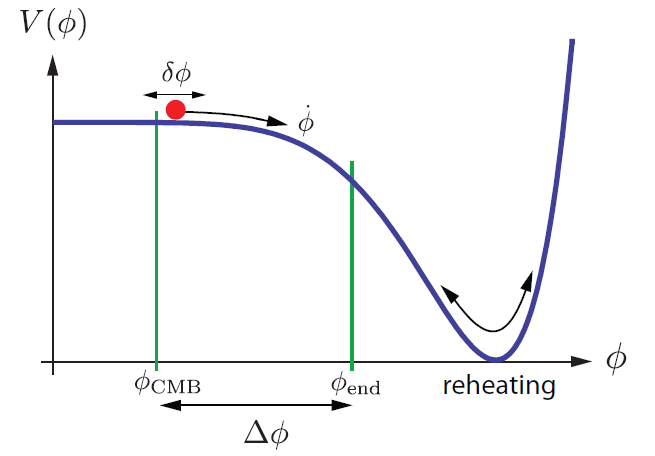
\includegraphics[width=0.7\textwidth]{Images/inflaton.png}
    \caption{A possible shape of the potential for Slow-Roll Inflation \cite{baumann2012tasi}}
    \label{fig:1.2} 
\end{figure}
\hspace{0.5cm} Let us try to understand under what conditions the scalar field may initiate inflation. The equation of motion for the homogeneous scalar field is given in Eq. \eqref{1.2.16}. To satisfy the condition given in Eq. \eqref{1.2.27} the scalar field should slowly roll down its potential. The easiest way to satisfy the slow roll condition is to require that there exist regions of field-configuration space where the potential is sufficiently flat. Considering the potential to be flat the acceleration of the field should be negligible i.e
\begin{align}
    \ddot{\varphi} \ll 3H\dot{\varphi} \label{1.2.29}
\end{align}
We can also say that at a sufficiently late time the scalar field is driven by friction term. Therefore,
\begin{align}
    3H\dot{\varphi} \approx -\partial_{\varphi} V \label{1.2.30}
\end{align}
We expect that $V$ and all of its derivatives change very slowly with $\varphi$.
This means that in this equation we have \(\partial_{\varphi} V \approx const\), as well as \(H \approx const\): this is the same equation that is obeyed by a particle under a constant force and friction: it will then reach the asymptotic ``{terminal velocity}'' and move with a constant \(\dot{\varphi}_0 \).\\ 

So, the slow-roll condition is,
\begin{align}
     \ddot{\varphi} \ll (3H\dot{\varphi}),(-\partial_{\varphi} V )\label{1.2.31}
\end{align}\\
Let us now combine it with the Friedmann equation  \eqref{eq:1.43},
\begin{align}
    H^2 = \frac{8 \pi G}{3} \qty(\rho _\varphi + \rho _m + \rho _r) - \frac{k}{a^2}\,.
\end{align}

The matter and radiation densities scale like \(a^{-3}\) for \(\rho _m\), \(a^{-4}\) for \(\rho _r\); in this early phase the scalar field dominates the dynamics, so the equation will simplify to 

\begin{align} \label{1.2.33}
    H^2 \approx \frac{8 \pi G}{3} V(\varphi)\,.
\end{align}
so, for a slow roll case, the Hubble parameter is nearly a constant and the scale factor is given by $a(t) \propto exp(Ht)$.\\
\hspace{0.5cm} We saw the slow roll conditions which are necessary for successful inflation. Next, we will parameterize it.

\
\hspace{0.5cm} These are the parameters we need to quantify in order to determine how closely the potential matches our expectations. It is given by $\epsilon$ and $\eta$. Let us start with the first parameter.\\
We define $\epsilon$ as,
\begin{align}
    \epsilon = -\frac{\dot{H}}{H^2}. \label{1.2.34}
\end{align}
As we saw previously for inflation to take place the Hubble radius shrinks. So let us write this in terms of the $\epsilon$ parameter.
\begin{align}
    \dv{(aH)^{-1}}{t} = \frac{-\dot{a}H + a\dot{H}}{(aH)^2} = -\frac{1}{a}\left( 1- \left( \frac{-\dot{H}}{H^2}\right)\right) = -\frac{1}{a}(1 - \epsilon) \label{1.2.35}
\end{align}
so we see that if $\dot{r_H} < 0$ implies that $\epsilon \ll 1 $.\\
\hspace{0.5cm} Using Eq. \eqref{1.2.30} and Eq. \eqref{1.2.33} we can write $\epsilon$ as,
\begin{align}
    \epsilon = - \frac{\dot{H}}{H^2} = + 4 \pi G \frac{\dot{\varphi}^2}{H^2} \approx \frac{3}{2} \frac{\dot{\varphi}^2}{V} = \frac{1}{16 \pi G} \qty(\frac{\partial_{\varphi} V}{V})^2\,,\label{1.2.36}
\end{align}
so the condition $\epsilon \ll 1 $ can also be written as 
\begin{align}
    \frac{(\partial_{\varphi} V)^2}{16 \pi G V^2} &\ll 1  \\ 
    \frac{(\partial_{\varphi} V)^2}{V} &\ll 16 \pi G V = \frac{2}{3} H^2 \\ 
    \frac{1}{V} \qty(\pdv{V}{\varphi })^2 &\ll H^2\,.\label{1.2.39}
\end{align}
on using Eq. \eqref{1.2.34} we can see that it is exactly the slow roll condition in Eq. \eqref{1.2.27}, So, we see that $\epsilon$ gives a bound on the first derivative of the potential and corresponds to the conditions of the potential being flat and the kinetic energy being small compared to the potential.\\
The second derivative of the potential is controlled by the parameter $\eta$ which is defined as,
 \begin{align}
     \eta = - \frac{\ddot{\varphi}}{H \dot{\varphi}}\,, \label{1.2.40}
 \end{align}
 and we can also define 

\begin{align}
    \eta = \frac{1}{3} \frac{\partial^{2} _{\varphi} V}{H^2} = \frac{1}{8 \pi G} \frac{\partial^{2} _{\varphi} V}{V} \,. \label{1.2.41}
\end{align}

We can see that \(\eta \ll 1 \) is equivalent to
\begin{align}
    \pdv[2]{V}{\varphi} \ll H^2 \label{1.2.42}
\end{align}

We can show that these three parameters are related  \(\delta = \eta - \epsilon \).\\
We start from Eq. \eqref{1.2.30} and differentiate it with respect to the time we get 

\begin{align}
    \ddot{\varphi} &\approx - \dv{}{t} \qty( \frac{\partial_{\varphi} V}{3H})  \\ &= - \frac{1}{3H} \partial^{2} _{\varphi} V \dot{\varphi} - \frac{\partial_{\varphi} V}{3} \underbracket{\qty(- \frac{\dot{H}}{H^2})}_{\epsilon }  \\ &= - \dot{\varphi} H \frac{\partial^{2} _{\varphi} V}{3H^2} - \frac{\partial_{\varphi} V}{3} \epsilon  \\ &= - \dot{\varphi} H \eta - \frac{\partial_{\varphi} V}{3} \epsilon  \\ {-\frac{\ddot{\varphi}}{H \ddot{\varphi}}} &= \eta - \epsilon  \\
    \delta &= \eta - \epsilon,.\label{1.2.48}
\end{align}
which is the desired result.
We see that $\delta \ll 1 $ corresponds to the condition $\ddot{\varphi} \ll -\partial_{\varphi} V$, which is required in order to neglect the acceleration term in the Klein-Gordon equation. So, the condition  $\delta \ll 1 $ ensures that we move towards an attractor solution in the friction-dominated regime i.e., it will then reach the asymptotic “terminal velocity” and move with a constant $\dot{\varphi}$. Also, for inflation to solve the horizon and the flatness problem we need a phase of accelerating expansion that lasts sufficiently long. For this to happen, we need $\epsilon \sim const$, since $\epsilon \sim \dot{\varphi}$ while $\delta \sim \ddot{\varphi}$, so requiring $\delta \ll 1$ also ensures this.
.\\
\hspace{0.5cm}In summary, the slow-roll approximation described in Eq. \eqref{1.2.27} and Eq. \eqref{1.2.31} implies the inflationary potential's flatness under conditions Eq. \eqref{1.2.36} and Eq. \eqref{1.2.41}.\\



\subsection{Inflation-Induced Cosmological Perturbations} \label{section 1.7.4}
 Inflationary cosmology relies on understanding the evolution of quantum fluctuations of the inflaton field $\delta \varphi(\mathbf{x},t)$, which give rise to primordial energy density perturbations that persist after inflation and form the basis of the large-scale structures observed in the Universe. These fluctuations arise on extremely small scales within the comoving Hubble radius during inflation, but the rapid expansion of space during this epoch stretches them out to cosmological scales. As the Hubble radius begins to increase faster than the scale factor after inflation ends, these fluctuations eventually re-enter the Hubble radius during the radiation or matter-dominated eras. The fluctuations that re-enter around 60 e-foldings before reheating have physical wavelengths that can be observed through various methods, such as the analysis of CMB anisotropies. The resulting inflationary spectrum provides a unique and distinct signature of inflation that can help us understand the origins of structure in the Universe. \\

 \begin{figure}[ht]
    \centering
    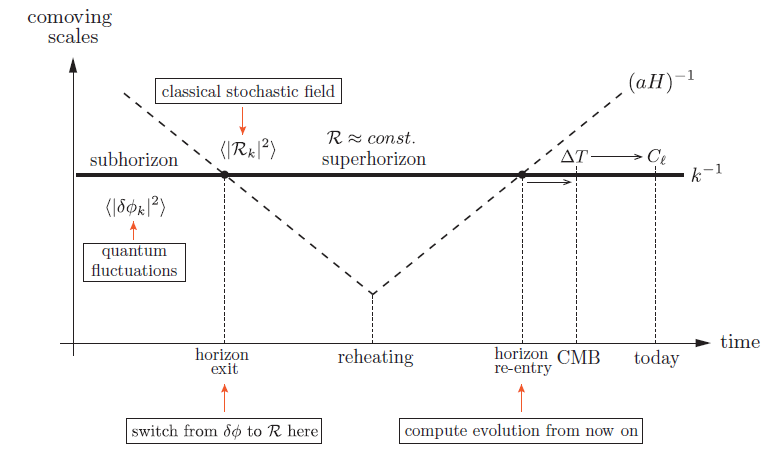
\includegraphics[width=0.7\textwidth]{Images/comving vs conformal time.png}
    \caption{Creation and evolution of perturbations in the inflationary universe. On subhorizon scales, quantum mechanics produces fluctuations. During inflation, comoving scales, $k^{-1}$, stay constant in the comoving Hubble radius, but  $(aH)^-{1}$ diminishes and the perturbations leave the horizon, where they remain frozen until horizon re-entry at later times. The fluctuations change into anisotropies in the CMB and disturbances in the LSS after horizon re-entry. Taken from \cite{baumann2012tasi}}
    \label{fig:1.3} 
\end{figure}

\subsubsection{Dynamics of Quantum Fluctuations: Qualitative Analysis}

 \hspace{0.5cm} Let us now describe qualitatively how the quantum fluctuations of a generic scalar field evolve during an inflationary stage. We saw the dynamics of the scalar field obey the Klein-Gordon Eq. \eqref{1.2.15} which we Taylor expand up to linear order around the background value for both $\varphi$ Eq. \eqref{1.2.23} and for the potential \(V(\varphi ) \approx V_0 + \delta \varphi \eval{(\pdv{V}{\varphi })}_{\varphi_0 }\). Assuming the perturbation is indeed small we can write the Klein-Gordon equation for the fluctuation as

\begin{align} 
    \ddot{ \delta \varphi} + 3 H \dot{\delta \varphi} - \frac{\nabla^2}{a^2} \delta \varphi = - \pdv[2]{V(\varphi )}{\varphi } \delta \varphi \,. \label{1.2.49}
\end{align}
Let us move to the Fourier space which is more convenient for the problem. We can write,
\begin{align}
    \delta \varphi (\mathbf{x}, t) = \frac{1}{(2\pi )^{3}} \int \dd[3]{k} 
    e^{i \mathbf{k} \cdot \mathbf{x}} \delta \varphi _{\mathbf{k}}(t)
    \,.\label{1.2.50}
\end{align}
Since the field is real, \(\delta \varphi _{\mathbf{k}} = \delta \varphi _{- \mathbf{k}}^{*}\).\\
Now we will write the Klein-Gordon equation for the quantum fluctuation in Fourier space.

\begin{align}
    \ddot{ \delta \varphi} _{\mathbf{k}} + 3 H \dot{ \delta \varphi}_{\mathbf{k}} + \frac{k^2}{a^2} \delta \varphi _{\mathbf{k}} = - \partial_{\varphi}^2(V) \delta \varphi _{\mathbf{k}}\,.\label{1.2.51}
\end{align}

If we consider a massless scalar field $\partial_{\varphi}^2(V) \approx 0$ which corresponds to the requirement of the parameter $\eta \ll 1$ which we discussed in the previous section. So, we can write the above equation as

\begin{align}
    \ddot{ \delta \varphi} _{\mathbf{k}} + 3 H \dot{ \delta \varphi}_{\mathbf{k}} + \frac{k^2}{a^2} \delta \varphi _{\mathbf{k}} \simeq 0 \label{1.2.52}
\end{align}\\

Now let us distinguish between the \textbf{sub-horizon}($\lambda < r_H$) and the \textbf{super-horizon}($\lambda > r_H$) regimes on the basis of the comoving wavelength $\lambda_{com} a(t) = \lambda_{physical} \simeq 2\pi/k_{physical}$

\begin{itemize}
    \item  \textbf{sub-horizon}($\lambda < r_H$):\\
    \begin{equation}
        \lambda \ll \frac{1}{aH} \implies \frac{k}{aH} \gg 1\ \label{1.2.53}
    \end{equation}
    We can write Eq. \eqref{1.2.52} as
    \begin{align}
        \ddot{ \delta \varphi} _{\mathbf{k}} + (3 H^2  + \frac{k^2}{a^2}) \delta \varphi _{\mathbf{k}} &=  \ddot{ \delta \varphi} _{\mathbf{k}} + \frac{k^2}{a^2} \delta \varphi _{\mathbf{k}} \simeq 0 \label{1.2.54}
    \end{align}  
    
    where we used the Hubble time scale \(t_{\mathrm{H}}=H^{-1}\) as the time reference and the sub-horizon condition Eq. \eqref{1.2.53}. So we observe that in the sub-horizon regime, the Fourier transform of the quantum fluctuations of the scalar field $\delta \varphi_{\mathbf{k}}$ can be described by a harmonic oscillator equation with a frequency term given by the factor $k / a(t)$ where the scale factor depends upon time as  \(a(t) \propto e^{Ht}\). This behaviour is expected, as at small scales inside the horizon, the local space-time appears flat like Minkowski space-time, and the expansion of the universe is negligible.
    
     \item  \textbf{super-horizon}($\lambda > r_H$):\\
    \begin{equation}
        \lambda \gg \frac{1}{aH} \implies \frac{k}{aH} \ll 1, \label{1.2.55}
    \end{equation}
    In this regime, we proceed as in the sub-horizon regime and observe that for the above condition given in Eq. \eqref{1.2.55}
    \begin{align}
       3 H^{2} \delta \varphi_{\mathbf{k}} \ll \frac{1}{a^{2}} k^{2} \delta \varphi_{\mathbf{k}} \label{1.2.56}
    \end{align}
    which shows that the friction term is dominant with respect to the Laplacian, therefore we can write Eq.\eqref{1.2.52} as
    \begin{align}
        \ddot{ \varphi_{\mathbf{k}}}+3 H \dot{\delta} \varphi_{\mathbf{k}} \simeq 0 \label{1.2.57}
    \end{align}    
    The solution for the above second-order differential Eq. \eqref{1.2.57} is given by
   \begin{align}
        \delta \varphi_{\mathbf{k}}=A+B e^{-3 H t} .
    \end{align}
    
    from this, we can interpret that as the exponential term decays and we get towards a constant fluctuation. In other words, as time increases the fluctuation oscillates until the wavelength gets larger than the Hubble horizon
    (maximum distance of causal connection), as soon as it is larger, the fluctuations can't interact nor grow and they cease to oscillate and get \emph{"frozen-in"}
\end{itemize}


\subsubsection{Dynamics of Quantum Fluctuations: exact solution}

In this section, we will discuss the exact solution to the dynamics of quantum fluctuation of a more generic scalar field \(\hat{\delta \varphi}(\tau, \mathbf{x}) \)  that includes quantum field theory effects and the mass term given by $\partial_{\varphi}^{2} V$. As done in the previous section, we explore the solution in the sub-horizon and super-horizon limits.

We start by redefining the field as,
\begin{align}
    \hat{\delta \varphi}(\tau, \mathbf{x})=a(\tau) \delta \varphi(\tau, \mathbf{x}) ,\
\end{align}

here we need to take into note that we are using conformal time $\tau$  instead of cosmic time. Now, we can write the generic scalar field  $\hat{\delta \varphi}(\tau, \mathbf{x})$ as a linear combination of the creation-annihilation operators $\left(a_{\mathbf{k}}, a_{\mathbf{k}}^{\dagger}\right)$

\begin{align}
    \hat{\delta \varphi}(\tau, \mathbf{x})=\frac{1}{(2 \pi)^{3}} \int \mathrm{d}^{3} \mathrm{k}\left[u_{\mathbf{k}}(\tau) a_{\mathbf{k}} e^{i \mathbf{k} \cdot \mathbf{x}}+u_{\mathbf{k}}^{*}(\tau) a_{\mathbf{k}}^{\dagger} e^{-i \mathbf{k} \cdot \mathbf{x}}\right]
\end{align}

and time-dependent mode functions $u_{\mathbf{k}}(\tau)$ that obeys a normalization condition
% In quantum field theory, a mode function describes the behaviour of a quantum field in terms of its wave-like properties. The normalization condition for a time-dependent mode function can be obtained by requiring that the total number of particles associated with the field is conserved.

\begin{align}
    u_{\mathbf{k}}^{\prime *}(\tau) u_{\mathbf{k}}(\tau)-u_{\mathbf{k}}^{*}(\tau) u_{\mathbf{k}}^{\prime}(\tau)= -i
\end{align}

such that commutation rules are given by


\begin{align}
    & {\left[a_{\mathbf{k}}, a_{\mathbf{k}^{\prime}}\right]=\left[a_{\mathbf{k}}^{\dagger}, a_{\mathbf{k}^{\prime}}^{\dagger}\right]=0,} \\
    & {\left[a_{\mathbf{k}}, a_{\mathbf{k}^{\prime}}^{\dagger}\right]=\hbar \delta^{(3)}\left(\mathbf{k}-\mathbf{k}^{\prime}\right) .}
\end{align}

In the Minkowski space-time the solutions i.e the mode functions are described by plane waves such as

\begin{align}
   u_{\mathbf{k}}(\tau) \sim \frac{e^{-i \omega_{\mathbf{k}} \tau}}{\sqrt{2 \omega_{\mathbf{k}}}}, \quad \omega_{\mathbf{k}}=\sqrt{k^{2}+m^{2}} .
 \end{align}


However, in the case of an expanding FRW Universe, we have a curved space-time, and we expect a more complicated expression for $u_{\mathbf{k}}(\tau)$. Since, in quantum field theory on curved space-time, the choice of the vacuum state is not unique enough to determine the mode functions due to the presence of the gravitational field. This means that different choices of vacuum state can result in different sets of mode functions, which can affect the physical properties of the theory. So, in short in quantum field theory on curved space-time there is an ambiguity with the choice of the vacuum state, therefore $u_{\mathbf{k}}(\tau)$ is not a priori fixed.\\
Looking at the equivalence principle as a guiding principle, modes \(u_{k} (\tau)\) at very short distances must reproduce the form for the ordinary flat space-time quantum field theory, which is the plane waves. So, we require  \begin{align}
    \frac{k}{aH} \rightarrow \infty \implies \  u_{\mathbf{k}}(\tau) \sim \frac{e^{-i \mathbf{k} \tau}}{\sqrt{2\mathbf{k}}}, \quad \sqrt{k^{2}+m^{2}} \simeq k  \label{1.2.65}   
\end{align}which is the Bunch-Davies condition on the vacuum state, which states that in the limit of small scales and for initial times the mode functions are given by
\begin{align}
    u_{\mathbf{k}}(\tau) \rightarrow \frac{e^{-i \mathbf{k} \tau}} {\sqrt{2\mathbf{k}}}. \label{1.2.66}
\end{align}
To motivate the inflationary vacuum state we try to recall our previous discussion that at a sufficiently early time all the modes of cosmological interest were deep inside the horizon i.e, which implies $k/aH \gg 1$ so, we can write $w_{k} \simeq k$ and there the mode function is given by Eq. \eqref{1.2.66}\\
\hspace{0.5cm} Before rewriting equation 1.2.45 in the Fourier space, we will explicitly change the time coordinate going from the reference time $t$ to the conformal time $\tau$ such that

\begin{align}
    \frac{d}{d t} \quad \longrightarrow \quad \frac{d}{d t} \frac{d \tau}{d \tau}=\frac{1}{a} \frac{d}{d \tau} \label{1.2.67}
\end{align}

let us perform the calculations term by term using the coordinate change in equation \eqref{1.2.67}. On the left-hand side of equation \eqref{1.2.51} we have


\begin{align}
    \delta \ddot{\varphi}_{\mathbf{k}} & =\frac{1}{a} \frac{d}{d \tau}\left[\frac{1}{a} \frac{d}{d \tau}\left(\frac{\delta \hat{\varphi}_{\mathbf{k}}}{a}\right)\right] \\
    & =\frac{1}{a} \frac{d}{d \tau}\left[\frac{1}{a}\left(\frac{\delta \hat{\varphi}_{\mathbf{k}}^{\prime}}{a}-\frac{a^{\prime}}{a^{2}} \delta \hat{\varphi}_{\mathbf{k}}\right)\right] \\
    & =\frac{1}{a}\left(\frac{\delta \hat{\varphi}_{\mathbf{k}}^{\prime \prime}}{a^{2}}-2 \frac{a^{\prime}}{a^{3}} \delta \hat{\varphi}_{\mathbf{k}}^{\prime}-\frac{a^{\prime \prime}}{a^{3}} \delta \hat{\varphi}_{\mathbf{k}}-3 \frac{a^{\prime 2}}{a^{4}} \delta \hat{\varphi}_{\mathbf{k}}-\frac{a^{\prime}}{a^{3}} \delta \hat{\varphi}_{\mathbf{k}}^{\prime}\right) \\
    & =\frac{\delta \hat{\varphi}_{\mathbf{k}}^{\prime \prime}}{a^{3}}-2 \frac{a^{\prime}}{a^{4}} \delta \hat{\varphi}_{\mathbf{k}}^{\prime}-\frac{a^{\prime \prime}}{a^{4}} \delta \hat{\varphi}_{\mathbf{k}}+3 \frac{a^{\prime 2}}{a^{5}} \delta \hat{\varphi}_{\mathbf{k}}-\frac{a^{\prime}}{a^{4}} \delta \hat{\varphi}_{\mathbf{k}}^{\prime},
\end{align}


and


\begin{align}
    3 H \delta \dot{\varphi}_{\mathbf{k}} & =3 \frac{1}{a^{2}} \frac{d a}{d \tau} \frac{1}{a} \frac{d}{d \tau}\left(\frac{\delta \hat{\varphi}_{\mathbf{k}}}{a}\right) \\
    & =3 \frac{a^{\prime}}{a^{4}} \delta \hat{\varphi}_{\mathbf{k}}^{\prime}-3 \frac{a^{\prime 2}}{a^{5}} \delta \hat{\varphi}_{\mathbf{k}}
\end{align}


Finally, putting all the results together, we obtain

\begin{align}
    \delta \hat{\varphi}_{\mathbf{k}}^{\prime \prime}-\frac{a^{\prime \prime}}{a} \delta \hat{\varphi}_{\mathbf{k}}+k^{2} \delta \hat{\varphi}_{\mathbf{k}}=-\partial_{\varphi}^{2} V a^{2} \delta \hat{\varphi}_{\mathbf{k}} \label{1.2.74}
\end{align}

which in terms of the mode functions can be written as

\begin{align}
    u_{\mathbf{k}}^{\prime \prime}(\tau)+\left(k^{2}-\frac{a^{\prime \prime}}{a}+\partial_{\varphi}^{2} V a^{2}\right) u_{\mathbf{k}}(\tau)=0 . \label{1.2.75}
\end{align}

 From this, we can see why we chose to use the re-scaled version  $\delta \hat{\varphi}_{\mathbf{k}}$. We can notice that the \emph{ansatz} is basically a harmonic oscillator with a time-dependent frequency changing according to the accelerated expansion of the universe. Let us look at the behaviour of the mode function in the sub-horizon and super-horizon regimes for a de Sitter Universe and a quasi-de Sitter Universe.

\subsubsection*{Solution in de-Sitter}
To solve the equation we will first consider the de-Sitter expansion where $H = constant$, $\epsilon \rightarrow 0$  and we assume the inflation is massless i.e 
\(m_{\varphi}^2 = \partial_{\varphi}^2{V} = 0\)
Under these conditions, we can write the  conformal time given by Eq. \eqref{eq:1.8} as

\begin{align}
    d \tau=\frac{d t}{a(t)}=d t e^{-H t} \label{1.2.76}
\end{align}

where we used the $a(t) \propto e^{Ht}$. After integration, we obtain the corresponding scale factor which reads as

\begin{align}
    a(\tau) = -\frac{1}{H\tau}(\tau < 0)  \label{1.2.77}
\end{align}
and
\begin{align}
    \frac{a''}{a} = 2a^2H^2 \label{1.2.78}
\end{align}

which on plugging it into Eq. \eqref{1.2.75} gives

\begin{align}
    u_{\mathbf{k}}^{\prime \prime}(\tau)+\left(k^{2}-2 a^{2} H^{2}\right) u_{\mathbf{k}}(\tau)=0 .\label{1.2.79}
\end{align}



In the \textbf{sub-horizon}($k \gg a H$) limit, Eq. \eqref{1.2.79} becomes

\begin{align}
    u_{\mathbf{k}}^{\prime \prime}(\tau)+k^{2} u_{\mathbf{k}}(\tau)=0 \quad \Rightarrow \quad u_{\mathbf{k}}(\tau)=\frac{e^{-i k \tau}}{\sqrt{2 k}} \label{1.2.80}
\end{align}


where we chose the Bunch-Davies vacuum state. As predicted in the qualitative analysis in the previous section, the behaviour of quantum fluctuations with wavelength within the cosmological horizon oscillates as we saw before in a flat space-time quantum field theory. This is what was expected for wavelengths much smaller than the Hubble radius scale where it is a good approximation to approximate the space-time as flat.\\

In the \textbf{super-horizon regime} ($k \ll aH$), Eq. \eqref{1.2.79} approximates as

\begin{align}
    u_{\mathbf{k}}^{\prime \prime}(\tau)-\frac{a^{\prime \prime}}{a} u_{\mathbf{k}}(\tau)=0 \label{1.2.81}
\end{align}



whose solution is simply given by

\begin{align}
    u_{\mathbf{k}}(\tau)=\underbracket{B(k) a(\tau)}_{\text{growing mode}}+ \underbracket{C(k) a(\tau)^{-2}}_{\text{decaying mode}} .\label{1.2.82}
\end{align}

 We see that the solution has a growing and a decaying mode where the decaying mode decays in time as $a(\tau)^{-2}$, so we can neglect the decaying mode because even if the amplitude increases it will decay quickly. Therefore the amplitude of the physical fluctuation reads as

\begin{align}
    \left|\delta \varphi_{\mathbf{k}}\right| \propto \frac{\left|u_{\mathbf{k}}\right|}{a(\tau)}=|B(k)| \label{1.2.83}
\end{align}

In the above equation, we can see that the “growing
mode” is actually asymptotically constant on super-horizon scales since $|B(k)|$ is independent of $\tau$.
To determine the scale of $B(k)$ we need to match the super-horizon and sub-horizon solutions, so it is basically a link between the quantum perturbation at horizon exit time during inflation and perturbation at horizon re-entry time during radiation or matter-dominated era. We thus evaluate $|B(k)|$ at the time of horizon crossing during inflation and we get

\begin{align}
    \abs{B(k)} a &= \abs{\frac{e^{-ik \tau }}{\sqrt{2 k}}} \label{1.2.84}  \\
    \abs{ \delta \varphi _\textbf{k}} &= \abs{B(k)} = \frac{1}{a \sqrt{2k}} 
    = \frac{H}{\sqrt{2 k^3}}\label{1.2.85}
    \,.
\end{align}

The fluctuation gets ``frozen in'' at horizon crossing: 

\begin{align}
    \abs{ \delta \varphi _\textbf{k}} = \frac{H}{\sqrt{2 k^3}}
    \,.
\end{align}

 Without proof, we will state the following result: the exact solution for the perturbation growth in De Sitter space-time is 

\begin{align}
     u_{\mathbf{k}}(\tau ) &= \frac{e^{ik \tau }}{\sqrt{2 k}} \qty(1 - \frac{i}{k \tau })
    \,.
\end{align}

As shown above, the physics underlying small scales below the horizon is described by special relativity, while quantum fluctuations around the vacuum expectation value of the scalar field are treated using quantum field theory in flat space-time. These fluctuations have a mean value of zero due to the nature of the vacuum state, which is characterized by the creation and annihilation of particles with a net number of particles equal to zero.

During inflation, the comoving Hubble radius shrinks, causing the rapid expansion to stretch the wavelength of the quantum fluctuations. This results in all fluctuations generated at sub-horizon scales exiting the horizon, where their amplitudes become frozen and are not affected by causal contact. After inflation ends, the comoving horizon begins to grow again, causing all fluctuations to re-enter the horizon with an imprint of their primordial fluctuations generated by inflation but with a much larger physical wavelength.

\subsubsection*{Solution in Quasi- de Sitter}
In this section, we will see how to solve the equation \eqref{1.2.75} explicitly 

\begin{align}
    u''_{\mathbf{k}} (\tau )
    + 
    \qty[k^2 - \frac{a''}{a} + a^2 m^2]  u_{\mathbf{k}}(\tau ) = 0\label{1.2.88}
    \,,
\end{align}

where \(\tau \) is the conformal time, while \(m^2 = \pdv*[2]{V}{\varphi }\). 
The stage in which \(m^2 = 0\) is the quasi-de-Sitter stage. 
Now we will consider that \(H\) is not a constant, instead, we will consider the effect of a nonzero slow-roll parameter \(\epsilon = - \dot{H} / H^2 \ll 1\). 
.We will use the relation
\begin{align}
    \frac{\ddot{a}}{a} = H^2 ( 1- \epsilon ) \label{1.2.89}
    \,,
\end{align}
which can be proven by straightforward manipulation.\\

Using the definition of the conformal time, we can show that the scale factor for small values of $\epsilon$ becomes

\begin{align}
    \tau = - \frac{1}{a H (1 - \epsilon )}\label{1.2.90}
\end{align}
\
 
Using this, we find that to first order 
\begin{align}
    (aH)^2 \approx (1 + 2 \epsilon ) / \tau^2 \label{1.2.91}
\end{align}
therefore we can re-write Eq. \eqref{1.2.89}  using Eq. \eqref{1.2.91} in terms of conformal time as,

\begin{align}
    \frac{a''}{a} = a^2 H^2 (2- \epsilon ) 
    =2 \frac{(1 + 2 \epsilon)}{\tau^2} \qty(1 - \frac{\epsilon}{2})
    \approx \frac{2}{\tau^2} \qty(1 + \frac{3}{2} \epsilon ) \label{1.2.92}
    \,.
\end{align}

Substituting this for \(a'' /a\) the equation becomes 

\begin{align}
    u''_{\mathbf{k}}(\tau ) + \qty[k^2 - \frac{\nu^2 - 1/4}{\tau^2}]  u_{\mathbf{k}}(\tau )= 0 \,,\label{1.2.93}
\end{align}

where \(\nu^2 = 9/4 + 3 \epsilon \). 
This is a Bessel equation: these equations are generally in the form 

\begin{align}
    z^2 y'' (z) + z y' (z) + (z^2 - \nu^2) y(z) = 0\,.
\end{align}

The solutions are called Hankel functions, assuming \(\nu\) as constant the general solution is given as

\begin{align}
     u_{\mathbf{k}}(\tau ) = \sqrt{- \tau } \qty[ c_1 (k) H_\nu^{(1)} (-k\tau ) + c_2 (k) H_\nu^{(2)} (-k\tau )] \,\label{1.2.95}
\end{align}

where \(H^{(2)}_\nu = H^{(1)*}_\nu\). 
We want to impose the asymptotic behaviour of the solution: let us start with 
\begin{itemize}
    \item \textbf{Sub-horizon (\(k / aH \gg 1\)):}\\ . 
    This means that 
    
    \begin{align*}
         u_{\mathbf{k}}(\tau ) = \frac{1}{\sqrt{2k}} e^{-ik \tau }
        \,,
    \end{align*}
        
    
    
    and the asymptotics of the Hankel functions are
    
    \begin{align}
        H^{(1)}_\nu  (x) \sim \sqrt{ \frac{2}{\pi x}} \exp(i \qty(x - \frac{\pi}{2} \nu - \frac{\pi}{4})) \sim \frac{e^{ix}}{\sqrt{x}} \, \label{1.2.96}
    \end{align}
    
    for \(x \gg 1\). This works well for us: we can set \(c_2 (k) = 0\) and only use \(c_1 (k)\). 
    
    We must choose 
    
    \begin{align}
        c_1 (k) = \frac{\sqrt{\pi }}{2} \exp(i \qty(\nu + \frac{1}{2}) \frac{\pi}{2})\,\label{1.2.97}
    \end{align}
    
    in order to have the correct normalization. 
    Then, our solution will read 
    
    \begin{align}
         u_{\mathbf{k}}(\tau ) = \frac{\sqrt{\pi }}{2} \exp(i ( \nu + \frac{1}{2}) \frac{\pi}{2}) \sqrt{-\tau } H^{(1)}_\nu (- k \tau )
        \,,\label{1.2.98}
    \end{align}
    \item \textbf{Super-horizon (\(k /aH \ll 1\)):}\\
    We have the asymptotic \(x \ll 1\) expansion of the Hankel function:

    \begin{align}
        H^{(1)}_\nu (x) \sim \sqrt{ \frac{2}{\pi }} e^{- i \pi /2}
        2^{\nu - 3/2} \frac{\Gamma (\nu )}{\Gamma (3/2)} x^{-\nu } \sim x^{-\nu }
        \,,\label{1.2.99}
    \end{align}
    
    therefore 
    
    \begin{align}
         u_{\mathbf{k}}(\tau ) \approx \exp(i (\nu - \frac{1}{2}) \frac{\pi}{2})
        2^{\nu - 3/2}
        \frac{\Gamma (\nu )}{\Gamma (3/2)}
        (- k \tau )^{1/2 - \nu } \frac{1}{\sqrt{2 k}} 
        \,,\label{1.2.100}
    \end{align}
\end{itemize}

so for getting the modulus \(\abs{ \delta \varphi _{\mathbf{k}}} = \abs{ u_{\mathbf{k}}} / a\) we can  use the fact that \(\tau \sim - 1/aH\), therefore \(\abs{ \delta \varphi _k} \approx - H \tau \abs{u_k}\). 
Inserting the expression we have for \(u_k\) we get,\footnote{Expanded to first order in \(\epsilon \), so that \(3/2 - \nu \approx - \epsilon \).}

\begin{align}
    \abs{ \delta \varphi _{\mathbf{k}}} 
    &\approx 2^{\nu - 3/2} \frac{\Gamma (\nu )}{\Gamma (3/2)} \frac{H}{\sqrt{2 k^3}} \qty(\frac{k}{aH})^{3/2 - \nu } \label{1.2.101} \\
    &\approx \frac{H}{\sqrt{2 k^3}} \qty( \frac{k}{aH})^{3/2 - \nu }
    \approx \frac{H}{\sqrt{2 k^3}} \qty( \frac{k}{aH})^{-\epsilon },\label{1.2.102}
\end{align}

which holds at super-horizon scales. In the De Sitter case, the exact result reads

\begin{align}
 u_{\mathbf{k}}(\tau ) \propto \sqrt{- \tau } H^{(1)}_{3/2} (- k \tau )
= \frac{e^{-ik \tau }}{\sqrt{2k}} \qty(1 - \frac{i}{k \tau })
\,.\label{1.2.103}
\end{align}\\

% The next step is to generalize to a scalar field that is not massless anymore: we shall consider a mass $m^2 = \frac{\partial^2 V}{\partial \varphi^2} \ll H^2$, so a "light" scalar field. We require this because one of the slow-roll parameters is $\eta_V = \frac{m^2}{3H^2} \ll 1$: a massive field (compared to $H^2$) would not be able to drive slow-roll inflation. 

% Then, the \(m^2 a^2\) term in the equation is nothing but 
% The next step is to generalize to a scalar field that is not massless anymore: we shall consider a mass $m^2 = \frac{\partial^2 V}{\partial \varphi^2} \ll H^2$, so a "light" scalar field. We require this because one of the slow-roll parameters is $\eta_V = \frac{m^2}{3H^2} \ll 1$: a massive field (compared to $H^2$) would not be able to drive slow-roll inflation.

% Then, the $m^2 a^2$ term in the equation is nothing but the mass term of the scalar field in an expanding universe. Since we are considering a "light" scalar field with a mass much smaller than the Hubble parameter, this term is much smaller than the $H^2$ term and can be neglected during inflation. This allows the scalar field to slowly roll down its potential, driving inflation. The slow-roll parameter $\eta_V$ is a measure of how much the scalar field's mass affects inflation, and a small value of $\eta_V$ is necessary for inflation to occur.
\hspace{0.5cm}Let's take a step forward in generalizing the scalar field with non-zero mass, denoted by $m^2 = \frac{\partial^2 V}{\partial \varphi^2}$. We require this mass to be much smaller than the Hubble parameter, $H$. This condition ensures that the scalar field can drive inflation through slow-roll. Specifically, we need the slow-roll parameter $\ \eta_V = \frac{m^2}{3H^2} \ll 1$.

The reason for this requirement is that a massive scalar field (compared to $H^2$) would not be able to maintain the slow-roll conditions needed for inflation. In other words, its mass would dominate over the Hubble friction term and prevent the scalar field from smoothly rolling down its potential.

 Then, the \(m^2 a^2\) term in the equation represents the mass term of the scalar field in an expanding universe which can be written as
\begin{align}
    m^2 a^2 = 3 \eta a^2 H^2 = \frac{3 \eta}{\tau^2}\label{1.2.104}
    \,,
\end{align}

but we also know that 

\begin{align}
    \frac{a''}{a} = \frac{2}{\tau^2 } \qty[ 1 + \frac{3}{2} \epsilon ]
    \,, \label{1.2.105}
\end{align}
%
Hence, the equation can still be recast into the same Bessel form but this time only the coefficient of the \(\tau^{-2}\) term changes.

The equation will read 
%
\begin{align}
    u''_{\mathbf{k}} (\tau ) + \qty[ k^2 - \frac{\nu^2 - 1/4}{\tau^2}]  u_{\mathbf{k}}(\tau ) = 0
    \,,\label{1.2.106}
\end{align}
%
with \(\nu^2 = 9/4 + 3 \epsilon - 3 \eta\). 
Then, the solution has exactly the same form as before:\\
on super-horizon scales, with \(k \ll aH\), we have
%
\begin{align}
    \abs{ \delta \varphi _k} = \frac{H}{\sqrt{2 k^3}} \qty( \frac{k}{aH})^{3/2 - \nu }
    &&
    \nu \approx \frac{3}{2} + \epsilon - \eta
    \,.\label{1.2.107}
\end{align}

It's worth noting that the previous computation doesn't only apply to an inflaton field, but also to any scalar field evolving during this phase of the universe's expansion. However, it's important to consider the field's mass - it can be shown that if $m^2$ is much greater than $H^2$, the super-horizon fluctuations of the field will have difficulty being excited and the field will remain in its vacuum state. So, if it's another scalar field, it needs to be light to be able to generate super-horizon fluctuations.








\subsection{The Power Spectrum} \label{section 1.7.5}
The power spectrum is a useful quantity to characterize the statistical properties of a Gaussian perturbation field which helps us to connect theoretical predictions with observational.\footnote{Perturbations close to Gaussian.}

The properties of a Gaussian random field $\delta(t, \mathbf{x})$ that represents a fluctuation in a point of space-time, such as the density fluctuation, can be described by an infinite set of correlation functions. These functions are defined as:

\begin{align}
    &\xi\left(\mathbf{x}_{1}, \mathbf{x}_{2}\right)= \left\langle\delta\left(t, \mathbf{x}_{1}\right) \delta\left(t, \mathbf{x}_{2}\right)\right\rangle, \label{1.2.108}\\
    &\xi\left(\mathbf{x}_{1}, \mathbf{x}_{2}, \mathbf{x}_{3}\right) = \left\langle\delta\left(t, \mathbf{x}_{1}\right) \delta\left(t, \mathbf{x}_{2}\right) \delta\left(t, \mathbf{x}_{3}\right)\right\rangle, \\
    & \vdots \\
    &\xi\left(\mathbf{x}_{1}, \mathbf{x}_{2}, \ldots, \mathbf{x}_{N}\right) =\left\langle\delta\left(t, \mathbf{x}_{1}\right) \delta\left(t, \mathbf{x}_{2}\right) \ldots \delta\left(t, \mathbf{x}_{N}\right)\right\rangle,
\end{align}


where the $\langle\cdot\rangle$ symbol refers to the ensemble average.

In the case of Gaussian random fields, they are determined by the two-point correlation function, i.e. the first definition in equation \eqref{1.2.108}. For reflection-symmetric Gaussian processes, the correlation function for odd $N$ is identically zero, whereas those characterized by even $N$ can be written as a combination of $\xi\left(\mathbf{x}_{1}, \mathbf{x}_{2}\right)$.\\
 The homogeneity condition implies that the statistical properties of the field are the same at every point in space. This means that the two-point correlation function, which characterizes the statistical dependence between two points in space, should only depend on the distance between the two points and not on their absolute positions. The isotropy condition applied to the two-point correlation function means that it should be invariant under spatial rotations. This implies that it should only depend on the magnitude of the separation vector between two points, and not on its direction. Therefore, the correlation function should only depend on the relative distance, and not on the relative orientation or direction of the separation vector between the two points $\xi(r)=\xi\left(\left|\mathbf{x}_{1}-\mathbf{x}_{2}\right|\right)$.

Knowing that the Fourier transform of the fluctuation reads as

\begin{align}
    \delta(t, \mathbf{x})=\frac{1}{(2 \pi)^{3}} \int \mathrm{d}^{3} k e^{i \mathbf{k} \cdot \mathbf{x}} \delta_{\mathbf{k}}(t) \label{1.2.112}
\end{align}



we define the power spectrum $P(k)$ as

\begin{align}
    \left\langle\delta_{\mathbf{k}_{1}}(t) \delta_{\mathbf{k}_{2}}(t)\right\rangle=(2 \pi)^{3} \delta^{(3)}\left(\mathbf{k}_{1}+\mathbf{k}_{2}\right) P(k), \label{1.2.113}
\end{align}



and we show that the power spectrum is the Fourier transform of the two-point correlation function $\xi(r)$. In fact


\begin{align}
    \xi(r) & =\langle\delta(t, x+r) \delta(t, x)\rangle \\
    & =\left\langle\frac{1}{(2 \pi)^{3}} \int \mathrm{d}^{3} k e^{i \mathbf{k} \cdot(\mathbf{x}+\mathbf{r})} \delta_{\mathbf{k}}(t) \frac{1}{(2 \pi)^{3}} \int \mathrm{d}^{3} k^{\prime} e^{i \mathbf{k}^{\prime} \cdot \mathbf{x}} \delta_{\mathbf{k}^{\prime}}(t)\right\rangle \\
    & =\frac{1}{(2 \pi)^{6}} \int \mathrm{d}^{3} k \int \mathrm{d}^{3} k^{\prime} e^{i \mathbf{k} \cdot(\mathbf{x}+\mathbf{r})} e^{\mathbf{k}^{\prime} \cdot \mathbf{x}}\left\langle\delta_{\mathbf{k}}(t) \delta_{\mathbf{k}^{\prime}}(t)\right\rangle \\
    & =\frac{1}{(2 \pi)^{3}} \int \mathrm{d}^{3} k \int \mathrm{d}^{3} k^{\prime} e^{i \mathbf{k} \cdot(\mathbf{x}+\mathbf{r})} e^{i \mathbf{k}^{\prime} \cdot \mathbf{x}} \delta^{(3)}\left(\mathbf{k}+\mathbf{k}^{\prime}\right) P(k) \\
    & =\frac{1}{(2 \pi)^{3}} \int \mathrm{d}^{3} k e^{i \mathbf{k} \cdot \mathbf{r}} P(k) . \label{1.2.118}
\end{align}
The plus is there since we wrote $\delta(k)\delta(k')$ instead of $\delta(k)\delta^*(k')$: if we included the conjugate then the argument of the $\delta$ would be $k-k'$, due to the fact that since $\delta(x)$ is real we have $\delta^*(k) = d(-k)$.

Another relevant quantity is the variance of the fluctuations defined as

\begin{align}
    \sigma^{2} \equiv\left\langle\delta_{\mathrm{k}}^{2}\right\rangle=\frac{1}{(2 \pi)^{2}} \int \mathrm{d}k k^2 P(k)  \label{1.2.119}
\end{align}



We further introduce the dimensionless power spectrum

\begin{align}
    \mathcal{P}(k) \equiv \frac{k^{3}}{2 \pi^{2}} P(k), \label{1.2.120}
\end{align}



by which Eq. \eqref{1.2.119} becomes

\begin{align}
    \sigma^{2}=\int_{0}^{\infty} \frac{\mathrm{d} k}{k} \mathcal{P}(k) \label{1.2.121}
\end{align}



The scale dependence of $\mathcal{P}(k)$ is given by the spectral index

\begin{align}
    n_{s}(k)-1=\frac{d \ln \mathcal{P}(k)}{d \ln k} . \label{1.2.122}
\end{align}



If the spectral index is scale-invariant, i.e. $n_{s}=$ const, then the power spectrum $\mathcal{P}(k)$ can be generally written as

\begin{align}
    \mathcal{P}(k)= \mathcal{A}_{s}\left(\frac{k}{k_{0}}\right)^{n_{s}-1}, \label{1.2.123}
\end{align}

where $k_{0}$ is a pivot scale. A useful way to categorize different power spectra is through the spectral index, denoted by $n_s$. The Harrison-Zel'dovich power spectrum, corresponding to $n_s=1$, is scale-invariant and does not depend on the cosmological scale $k$ and $\mathcal{A}_{s} =\mathcal{P}(k_{0})$ . A blue-tilted power spectrum, with $n_s>1$, implies that perturbations have more power on small scales than on large scales. Conversely, a red-tilted power spectrum, with $n_s<1$, indicates that there is less power on small scales compared to large scales.
The power spectrum of the fluctuations of the inflaton field at lowest order in the slow-roll parameters. Using the fact that $\delta \varphi_{\mathbf{k}}(t)^{*}=\delta \varphi_{-\mathbf{k}}(t)$ and that it can be written as a combination of creation-annihilation operators
\footnote{Writing the L.H.S of \eqref{1.2.124} in terms of creation and annihilation operators: we have $$\bra{0} a a \ket{0}=\bra{0} a ^\dag a  \ket{0}= \bra{0} a ^\dag a ^\dag \ket{0}= 0 \,,$$
while $$\bra{0} a a ^\dag \ket{0} = \underbracket{\bra{0} \qty[a, a ^\dag] \ket{0}}_{\delta^{(3)} (\mathbf{k} - \mathbf{k'})} - \underbracket{\bra{0} a ^\dag \ket{0}}_{= 0} \,$$
so,
$$
\expval{ \delta \varphi _{\mathbf{k}} \delta \varphi _{\mathbf{k'}}^{*}} = (2 \pi )^3 \abs{ \delta \varphi _{\mathbf{k}}}^2 \delta^3(\mathbf{k} -\mathbf{k'})\
$$
}
we obtain

\begin{align}
    \left\langle\delta \varphi_{\mathbf{k}}(t) \delta \varphi_{\mathbf{k}^{\prime}}^{*}(t)\right\rangle=(2 \pi)^{3} \delta^{(3)}\left(\mathbf{k}-\mathbf{k}^{\prime}\right)\left|\delta \varphi_{\mathbf{k}}\right|^{2} .\label{1.2.124}
\end{align}

Comparing this result with equation \eqref{1.2.113} we have 

\begin{align}
    P_{\delta \varphi}(k)=\left|\delta \varphi_{\mathbf{k}}(t)\right|^{2}, \quad \mathcal{P}_{\delta \varphi}(k)=\frac{k^{3}}{2 \pi^{2}}\left|\delta \varphi_{\mathbf{k}}\right|^{2} .\label{1.2.125}
\end{align}\\

In particular, using the result in \eqref{1.2.107} we find that at super-horizon scales the power spectrum reads as

\begin{align}
    \mathcal{P}_{\delta \varphi}(k)=\left(\frac{H}{2 \pi}\right)^{2}\left(\frac{k}{a H}\right)^{3-2 \nu} .\label{1.2.126}
\end{align}

\subsection{From Quantum to Cosmological Fluctuations}
During inflation, the inflaton field fluctuations $\delta \varphi$ arise at sub-horizon scales and are stretched by the rapid expansion of the Universe until they exit the horizon and freeze at super-horizon scales, as shown in section \eqref{section 1.7.4}. Later on, these fluctuations re-enter the region of causal connection and interact through physical processes. In this section, we investigate how the quantum perturbations during inflation relate to the primordial density perturbations that act as the seeds for the current cosmic structure.

Due to the presence of these fluctuations, different regions of the Universe complete inflation at slightly different times. This is demonstrated by considering the equation of motion of the homogeneous inflaton field \eqref{1.2.16} and splitting the scalar field as 
\begin{align}
    \varphi (\mathbf{x}, t) = \varphi_0 (t) + \delta \varphi (\mathbf{x}, t)
    \,, \label{1.2.127}
\end{align}
Now taking its derivative with respect to cosmic time we get

\begin{align}
    \dddot{\varphi} + 3H\ddot{\varphi} = -\partial_{\phi}^2 V(\varphi)\dot{\varphi} &\implies \partial_{t}^2 {(\dot{\varphi})} + 3H\partial_{t}{(\dot{\varphi})} = - \partial_{\phi}^2 V(\varphi)\dot{\varphi}\label{1.2.128}
\end{align}

we notice that the resulting equation has the same form as Eq. \eqref{1.2.51} except for the Laplacian term. In the limit where this term can be neglected, $\delta \varphi$ and $\varphi$ obey the same equation. In particular, taking the Fourier transform of the Laplacian term

\begin{align}
    \frac{1}{a^{2}} \nabla^{2}(\delta \varphi) \stackrel{\mathcal{F}}{\rightarrow}-\frac{k^{2}}{a^{2}} \delta \varphi_{\mathbf{k}}\label{1.2.129}
\end{align}

we have that it vanishes in the limit of large scales, i.e. for $k$ that tends to 0. This implies that the Laplacian term can be ignored on large scales, and we can assume a coarse-graining process that is valid for the discussion of inflationary fluctuations.

The Wronskian operator, a mathematical tool that enables us to determine whether a group of solutions to a differential equation are linearly independent or linearly dependent, is used to analyze this system. Given two homogeneous fields $\varphi(t)$ and $\psi(t)$, the Wronskian is defined as

\begin{align}
    W(\varphi, \psi)=\dot{\varphi} \psi-\dot{\psi} \varphi \begin{cases}\neq 0 & \text { two linearly independent solutions, } \\ =0 & \text { two linearly dependent solutions. }\end{cases} \label{1.2.130}
\end{align}

In our case, the Wronskian has the following form

\begin{align}
   W(\dot{\varphi_0}, \delta \varphi ) &= \ddot{\varphi_0} \delta \varphi - \dot{\varphi_0} \dot{ \delta \varphi}\,.\label{1.2.131}
\end{align}

If we further derive with respect to time, we obtain that


\begin{align}
    \dot{W} &= \dot{\ddot{\varphi}}_0 \delta \varphi + \ddot{\varphi}_0 \dot{ \delta \varphi} - \ddot{\varphi}_0 \dot{\delta \varphi } - \dot{\varphi}_0 \ddot{\delta \varphi }  \\
    &= \delta \varphi \qty(- 3H \ddot{\varphi}_0 - V'' \dot{\varphi}_0 ) - \dot{\varphi}_0 \qty(- 3H \dot{\delta \varphi } - V'' \delta \varphi )  \\
    &= - 3H \qty(\ddot{\varphi_0} \delta \varphi - \dot{\varphi_0} \dot{ \delta \varphi}) = -3HW(\dot{\varphi_0}, \delta \varphi )\label{1.2.134}
    \,.
\end{align}

which has a solution decaying with time given by

\begin{align}
    W(\dot{\varphi_0}, \delta \varphi )=e^{-3 H t}\label{1.2.135}
\end{align}

Thus, using the conditions \eqref{1.2.130}, at large scales $\delta \varphi$ and $\dot{\varphi_0}$ are related. In particular

\begin{align}
    \delta \varphi(t, \mathbf{x}) \propto \dot{\varphi_0} \Rightarrow \delta \varphi(t, \mathbf{x}) \simeq(-\delta t(\mathbf{x})) \dot{\varphi_0}\label{1.2.136}
\end{align}

where the proportional constant $-\delta t(\mathbf{x})$ must have the dimensionality of time as $\delta \varphi(t, \mathbf{x})$is space dependent($\mathbf{x}$ that represents a large region of the Universe) whereas $\dot{\varphi_0}$ is not.So, by reverse-Taylor expansion, the full field is given by


\begin{align}
    \varphi(t, \mathbf{x}) & =\varphi_{0}(t)+\delta \varphi(t, \mathbf{x}) \label{1.2.137}\\
    & \simeq \varphi_{0}[t-\delta t(\mathbf{x})] .\label{1.2.138}
\end{align}
The inflaton field is subject to a temporal shift given by

\begin{align}
\delta t(\mathbf{x}) \simeq-\frac{\delta \varphi(t, \mathbf{x})}{\dot{\varphi}(t)}\label{1.2.139}
\end{align}


The expression \eqref{1.2.138} tells us that at each point in space $\mathbf{x}$, the field $\varphi$ takes on the same values as the field $\varphi_{0}$ at a slightly earlier time $t-\delta t(\mathbf{x})$. In other words, the value of the field at each point evolves in time, but the evolution is slightly delayed at each point. This is because the field at each point feels the influence of its surroundings, and fluctuations in the surrounding field cause the field at that point to evolve differently than if it were completely isolated.

This interpretation is intuitive if we consider the analogy of waves on a water surface. Imagine that we drop a pebble in the middle of a still pond, creating a circular wave pattern. As the waves propagate outward, the shape of the wave pattern at any point in the pond depends on the position and shape of the waves at all other points. Similarly, in a fluctuating field like $\varphi$, the value of the field at any point depends on the values of the field at all other points.\

In this sense, the delayed evolution of the field at each point can be thought of as a result of the time it takes for information to propagate through the field. Information about fluctuations in the field has to propagate from one point to another, and this takes time. Therefore, the evolution of the field at each point is slightly delayed relative to the evolution of the field as a whole. As a consequence, also the expansion of the Universe is different in different parts of the Universe.\\ We introduce the fluctuations in the number of e-folds $\mathcal{N}$ Eq. \eqref{1.2.1} given by the primordial curvature perturbation \(\zeta\)

\begin{align}
    \zeta=\delta \mathcal{N}=H \delta t \simeq-H \frac{\delta \varphi}{\dot{\varphi}}\label{1.2.140}
\end{align}

where in the last passage we used Eq. \eqref{1.2.139}. We now show that during inflation the primordial curvature perturbation induces fluctuations in the density field. Let us consider the expression of $\rho$ in equation \eqref{1.2.25}, then


\begin{align}
    -H \frac{\delta \rho}{\dot{\rho}} & \simeq-H \frac{\partial_{\varphi} V(\varphi) \delta \varphi}{-3 H(\rho+p)}, \\
    & \simeq H \frac{3 H \dot{\varphi} \delta \varphi}{-3 H \dot{\varphi}^{2}} \simeq-H \frac{\delta \varphi}{\dot{\varphi}}, \label{1.2.142}
\end{align}


where in the first passage we used the continuity equation \eqref{eq:1.20c} during inflation. Therefore, $\zeta \simeq-H \delta \rho / \dot{\rho}$. An important property of $\zeta$ is that it remains constant outside the horizon for adiabatic matter perturbations\cite{Bartolo_2004}. Therefore, given a scale $k$, we can evaluate $\zeta$ at the time of horizon crossing $t(k)_{\text {exit }}$, knowing that it maintains the same value until it re-enters the horizon at $t(k)_{\text {enter}}$ during radiation or matter domination.

The power spectrum of the curvature perturbation can be derived using Eq. \eqref{1.2.140}
\begin{align}
    \mathcal{P}_{\zeta} \simeq \frac{H^{2}}{\dot{\varphi}^{2}} \mathcal{P}_{\delta \varphi}=\left(\frac{H^2}{2 \pi \dot{\varphi}}\right)^{2}\left(\frac{k}{a H}\right)^{3-2 \nu} \label{1.2.143}
\end{align}

and at the time of horizon exit ($k \approx aH$), we have



\begin{align}
    \mathcal{P}_{\zeta}=\left.\left(\frac{H^2}{2 \pi \dot{\varphi}}\right)^{2}\right|_{t(k)_{exit }} .\label{1.2.144}
\end{align}

The curvature perturbation $\zeta$ introduced in Eq.\eqref{1.2.140} is a particular form of the gauge-invariant curvature perturbation on uniform-density hyper-surfaces defined as

\begin{align}
    \zeta \equiv-\psi-H \frac{\delta \rho}{\dot{\rho}} \label{1.2.145}
\end{align}
where $\psi$ is the scalar perturbation of the diagonal spatial component of the FRW metric known as the Bardeen Potential. In fact, in Eq. \eqref{1.2.140} we considered the gauge choice $\psi=0$, called \textbf{uniform curvature gauge}.\\
To calculate the curvature perturbation on large scales we can consider the curvature perturbation on comoving surfaces which in the case of the scalar field reads as,
\begin{align}
    \mathcal{R}_c = \psi + H \frac{\delta \varphi}{\dot{\varphi}},\ \label{1.2.146}
\end{align}
which is the metric perturbation in the comoving space-time slicing(observer which sees the cosmic expansion as isotropic). It can be shown that both $\mathcal{R}_c$ and $\zeta$
are gauge invariant and on large scales they are equal,
\begin{align}
    \mathcal{R}_c = -\zeta = \psi + H \frac{\delta \varphi}{\dot{\varphi}},\ \label{1.2.147}
\end{align}
The scale index of the power spectrum can be parameterized using a scale dependence of the spectral index $n_s$ \eqref{1.2.123}:
\begin{align}
    \mathcal{P}_{\zeta}  = A_s (\frac{k}{k_0})^{n_s -1 + \frac{1}{2}\alpha_{s} ln(k/k_0)+ \frac{1}{3!}\beta_{s}ln^2(k/k_0) + ....},\ \label{1.2.148}
\end{align}
where $A_{s}$ is the scalar amplitude and the coefficients $\alpha_{s}$,$\beta_{s}$ are, respectively, called "running of spectral index" and "running of running"
parameters. They are independent of k and are obtained by Taylor expansion of the spectral index. In the slow roll approximation, we can write $\mathcal{P}_{\zeta}(k)$ as a function of the slow roll potential and its derivatives, hence we can write the running parameters as a function of the slow roll parameters\cite{baumann2012tasi}.\\
\begin{align}
    1-n_{s} = 2\eta - 6\epsilon \\
    \alpha_s = -2\xi^2 + 16\eta\epsilon - 24\epsilon^2 \\
    \beta_{s} = 2\sigma^3 + + 2\xi^2(\eta -12\epsilon) - 32\epsilon(\eta^2 - 6\eta\epsilon + 6 \epsilon^2) \label{1.2.149}.
\end{align}
In the standard slow-roll inflation models, $\alpha_s$ and $\beta_{s}$ are highly suppressed by slow-roll parameters. However, in the large-running mass inflation model, these parameters would be
relatively large.

\section{Primordial Non-Gaussianity} \label{PNG}

Previously, we saw that for a single field inflationary model, the action considered is that of a single field coupled to gravity Eq. \eqref{1.2.10} and the leading order term in this expansion is quadratic in the small fluctuations around the homogeneous background. Since a free field can be viewed as a collection of harmonic oscillators, and these oscillators begin in their ground state, the resulting fluctuations are Gaussian to the leading order. However, there can be deviations from the Gaussian initial conditions \cite{Maldacena_2003} when the conditions for the standard inflationary model are not met, like, in the case of the multi-field inflation \cite{Polarski_1994} or the curvaton scenario \cite{Lyth_2002}. For a detailed review of the generation of primordial non-Gaussianity (PNG) from different inflationary models refer to \cite{Bartolo_2004} and the references therein .\\

In the context of Gaussian random fields, all information is encapsulated in the power spectrum. The bispectrum, which is the Fourier transform of the three-point correlation function, is significant as it serves as the lowest-order statistic capable of distinguishing non-Gaussian features from Gaussian perturbations.\\

Each inflationary model makes specific predictions regarding the bispectrum of the primordial perturbations in the gravitational potential $\Phi_{\mathbf{k}}$ hence accurately calculating the primordial bispectrum of cosmological perturbations is a crucial area of research for enhancing our understanding of the early universe. The bispectrum $B_{\Phi}\left(k_{1}, k_{2}, k_{3}\right)$ of these perturbations is defined as:

\begin{equation}
    \left\langle\Phi\left(\mathbf{k}_{1}\right) \Phi\left(\mathbf{k}_{2}\right) \Phi\left(\mathbf{k}_{3}\right)\right\rangle \equiv(2 \pi)^{3} \delta_{D}\left(\mathbf{k}_{123}\right) B_{\Phi}\left(k_{1}, k_{2}, k_{3}\right) \label{eq:1.229}
\end{equation}

where  $\mathbf{k}_{i j} \equiv \mathbf{k}_{1}+\mathbf{k}_{2}$ so that the Dirac delta function here is $\delta_{D}\left(\mathbf{k}_{123}\right) \equiv \delta_{D}\left(\mathbf{k}_{1}+\mathbf{k}_{2}+\mathbf{k}_{3}\right)$. 
Together with the assumption of statistical homogeneity and isotropy for the primordial perturbations, this implies that the bispectrum is a function of the triplet defined by the magnitude of the wavenumbers $k_{1}, k_{2}$ and $k_{3}$ forming a closed triangular configuration.
Additionally. we can write

\begin{equation}
    B_{\Phi}\left(k_{1}, k_{2}, k_{3}\right) \equiv f_{\mathrm{NL}} F\left(k_{1}, k_{2}, k_{3}\right) \label{eq:1.230}
\end{equation}
where $F\left(k_{1}, k_{2}, k_{3}\right)$ encodes the functional dependence of the primordial bispectrum on the specific triangle configurations and $f_{NL}$ is the dimensionless PNG amplitude that measures the strength of the PNG signal.\footnote{"NL" stands for non-linear}

Predictions for both the amplitude $f_{\mathrm{NL}}$ and the functional dependence $F\left(k_{1}, k_{2}, k_{3}\right)$ vary significantly between different inflationary models. Below is a brief description of the three main templates of primordial bispectrum shapes. For more details refer to \cite{meerburg2019primordialnongaussianity} and references therein.

The parameter space of single-field models is well-described by the so-called equilateral and orthogonal templates.\cite{creminelli2006JCAP...05..004C, Chen_2007}


\begin{equation}
\begin{aligned}
    B_{\Phi}^{\text{equil}}\left(k_1, k_2, k_3\right) = 6 A^2 f_{\mathrm{NL}}^{\text{equil}} & \times\left\{-\frac{1}{k_1^{4-n_s} k_2^{4-n_s}} - \frac{1}{k_2^{4-n_s} k_3^{4-n_s}} - \frac{1}{k_3^{4-n_s} k_1^{4-n_s}} - \frac{2}{\left(k_1 k_2 k_3\right)^{2\left(4-n_s\right) / 3}}\right. \\
    & \left.\quad + \left[\frac{1}{k_1^{\left(4-n_s\right) / 3} k_2^{2\left(4-n_s\right) / 3} k_3^{4-n_s}} + 5 \text{ perms. }\right]\right\}
\end{aligned}
\label{eq:1.231}
\end{equation}

\begin{equation}
\begin{aligned}
    B_{\Phi}^{\text{ortho}}\left(k_1, k_2, k_3\right) = 6 A^2 f_{\mathrm{NL}}^{\text{ortho}} & \times\left\{-\frac{3}{k_1^{4-n_s} k_2^{4-n_s}} - \frac{3}{k_2^{4-n_s} k_3^{4-n_s}} - \frac{3}{k_3^{4-n_s} k_1^{4-n_s}} - \frac{8}{\left(k_1 k_2 k_3\right)^{2\left(4-n_s\right) / 3}}\right. \\
    & \left.\quad + \left[\frac{3}{k_1^{\left(4-n_s\right) / 3} k_2^{2\left(4-n_s\right) / 3} k_3^{4-n_s}} + 5 \text{ perms. }\right]\right\}
\end{aligned}
\label{eq:1.232}
\end{equation}

The bispectrum for multi-field models is typically of the local type(for a review refer \cite{Byrnes_2010}) given by 

\begin{equation}
    \begin{aligned}
        B_{\Phi}^{\text{local}}\left(k_1, k_2, k_3\right) = & \; 2 f_{\mathrm{NL}}^{\text{local}}\left[P_{\Phi}\left(k_1\right) P_{\Phi}\left(k_2\right) + P_{\Phi}\left(k_1\right) P_{\Phi}\left(k_3\right) + P_{\Phi}\left(k_2\right) P_{\Phi}\left(k_3\right)\right] \\
        = & \; 2 A^2 f_{\mathrm{NL}}^{\text{local}}\left[\frac{1}{k_1^{4-n_s} k_2^{4-n_s}} + \text{cycl.}\right].\label{eq:1.233}
    \end{aligned}
\end{equation}
To use non-Gaussianities as a probe of the early Universe and the details of inflation, it is essential to measure both the shape of the primordial bispectrum and the magnitude of its signal, specifically by constraining the $f_{NL}$  parameter. The detection of non-Gaussianities can provide a way to distinguish between the different classes of inflationary models and eliminate those that don’t predict
such an amount of deviation from the exact Gaussian distribution.


%%%%%%%%%%%%%%%%%%%%%%%%%%%%%%%%%%%%%%%%%%%%%%%%%%%%%%%%%%%%%%%%%%%%%%%%%%%%%%%%%%%
\section{Neutrino Mass} \label{neutrinos}
In section \ref{thermal history}, we discussed how neutrinos decoupled from the plasma in the early universe. These relic neutrinos leave detectable imprints on cosmological observations. The energy distribution and dynamics of these relic neutrinos have significant consequences for the evolution of the Universe.

Initially, the relic neutrinos were relativistic from the time of their decoupling through to recombination. Due to the expansion and cooling of the Universe, their momenta redshifted as $p_{\nu} \propto 1 / a$, eventually causing the energy of most relic neutrinos to be dominated by their rest mass rather than their momentum. Consequently, the energy density in non-relativistic neutrinos contributes to the matter budget of the Universe today. However, since neutrinos were relativistic for much of the Universe's history, their gravitational clustering differs qualitatively from that of cold dark matter (CDM) particles. This difference allows us to distinguish between the contributions of neutrinos and cold dark matter to the overall matter density \cite{LESGOURGUES_2006}. In this section, we review how neutrino mass affects the evolution of the neutrino energy density and the gravitational clustering of matter following \cite{LESGOURGUES_2006, abazajian2016cmbs4sciencebookedition}.

Current constraints from the cosmic microwave background (CMB) on $N_{\text{eff}}$ \cite{PLanck20182020} align closely with the Standard Model expectation of three species of neutrinos and antineutrinos, each described by a relativistic thermal Fermi-Dirac distribution. The distribution function for each species of neutrinos and antineutrinos is given by


\begin{equation}
    f_{\nu}(p) = \frac{1}{e^{a p / T_{\nu 0}} + 1} \label{n.1}
\end{equation}

where $T_{\nu 0} \approx 1.7 \times 10^{-4} \, \mathrm{eV} (1.95 \, \mathrm{K})$ is the temperature today \cite{ParticleDataGroup:2022pth}. In Standard Model physics, the spectral shape of the neutrino phase space distribution is preserved with the expansion, so relic neutrinos have retained the relativistic Fermi-Dirac momentum distribution inherited from decoupling even as the individual neutrinos became non-relativistic.

Now, we write the neutrino energy density as

\begin{equation}
    \rho_{\nu} = \sum_{i} \int \frac{d^{3} \mathbf{p}}{(2 \pi)^{3}} \frac{\sqrt{p^{2} + m_{\nu i}^{2}}}{e^{a p / T_{\nu 0}} + 1}
    \label{n.2}
\end{equation}

where $m_{\nu i}$ are the three neutrino mass eigenstates. For $T_{\nu} / a \gg m_{\nu i}$ the neutrino energies are dominated by their momenta and the total energy density behaves like radiation

\begin{equation}
    \left.\rho_{\nu}\right|_{\text{early}} \approx \frac{7 \pi^{2}}{40} \left(T_{\nu 0}\right)^{4} \frac{1}{a^{4}} \propto a^{-4}
    \label{n.3}
\end{equation}

While for $T_{\nu 0} / a \ll m_{\nu i}$ the energy density behaves like matter

\begin{equation}
    \left.\rho_{\nu}\right|_{\text{late}} \approx \sum_{i} m_{\nu i} \bar{n}_{\nu} \propto a^{-3}
    \label{n.4}
\end{equation}

where $\bar{n}_{\nu}$ is the number of neutrinos and antineutrinos in each mass eigenstate

\begin{equation}
    \bar{n}_{\nu} = \int \frac{d^{3} \mathbf{p}}{(2 \pi)^{3}} \frac{2}{e^{a p / T_{\nu 0}} + 1} \approx \frac{113}{a^{3}} \, \mathrm{cm}^{-3}
    \label{n.5}
\end{equation}

For a neutrino of mass $m_{\nu i}$, the transition between these two regimes $\left(k_{B} T_{\nu}(a) \sim m_{\nu i}^{2}\right)$ occurs at redshift $z_{\mathrm{nr}} \sim 300\left(m_{\nu i} / 0.05 \, \mathrm{eV}\right)$. Using Eq. \ref{n.4}, the fractional energy density in neutrinos today can be written as

\begin{equation}
    \Omega_{\nu} h^{2} \approx \frac{\sum_{i} m_{\nu i}}{93 \, \mathrm{eV}}
    \label{n.6}
\end{equation}

The individual masses of the neutrino states are unknown but neutrino oscillation data specifies the square of two mass splittings $\Delta m_{12}^{2} = 7.54 \times 10^{-5} \, \mathrm{eV}, \left|\Delta m_{13}^{2}\right| \approx 2.4 \times 10^{-3} \, \mathrm{eV}$ \cite{ParticleDataGroup:2014cgo}. These mass splittings, in combination with the neutrino number density, give a lower limit on the contribution of neutrinos to the cosmic energy budget \cite{abazajian2016cmbs4sciencebookedition}

\begin{equation}
    \Omega_{\nu} h^{2} \gtrsim 0.0006
    \label{n.7}
\end{equation}

At $z \ll z_{\mathrm{nr}}$, the matter density of the Universe, which enters into the Hubble equation, is the sum of the CDM, baryon, and massive neutrino energy densities $\Omega_{m} = \Omega_{c} + \Omega_{b} + \Omega_{\nu}$. Whereas, at $z \gg z_{\mathrm{nr}}$, the matter density is solely made up of the baryon and CDM parts while neutrinos contribute to the radiation density.

Neutrinos do not contribute to gravitational collapse until they transition to a nonrelativistic state. Before this transition, neutrinos free-stream out of gravitational wells, leaving behind cold dark matter (CDM) and baryons. As a result, primordial fluctuations in the neutrino density are damped on scales smaller than the horizon at $z_{\mathrm{nr}}$. In comoving coordinates, this scale is represented by a wave number.

\begin{equation}
    k_{\mathrm{nr}} \equiv a_{\mathrm{nr}} H\left(a_{\mathrm{nr}}\right) \approx 0.003 \left(\frac{\Omega_{m}}{0.3} \frac{m_{\nu}}{0.05 \, \mathrm{eV}}\right)^{1 / 2} \, h / \mathrm{Mpc}
\label{n.8}
\end{equation}

Once the neutrinos are non-relativistic, their finite velocity dispersion still prevents them from clustering on scales smaller than the typical distance a neutrino travels in a Hubble time, $v_{\nu} / H(a)$ where $v_{\nu} \approx 3.15 T_{\nu 0} /\left(a m_{\nu}\right)$ the mean neutrino velocity. In analogy with the Jeans criterion for gravitational collapse, the neutrino free-streaming scale is defined in comoving coordinates as

\begin{equation}
    k_{\mathrm{fs}}(a) \equiv \sqrt{\frac{3}{2}} \frac{a H(a)}{v_{\nu}(a)} \approx 0.04 a^{2} \sqrt{\Omega_{m} a^{-3} + \Omega_{\Lambda}}\left(\frac{m_{\nu}}{0.05 \, \mathrm{eV}}\right) \, h / \mathrm{Mpc}
    \label{n.9}
\end{equation}

On scales larger than $k_{\mathrm{nr}}$, adiabatic perturbations in the densities of neutrinos, baryons, and cold dark matter (CDM) are coherent and can be described by a single perturbation to the total matter density $\delta_{m} = \delta \rho_{m} / \rho_{m}$. On smaller scales, where neutrino perturbations have decayed, only perturbations in CDM and baryons remain, such that $\delta_{m} = \delta_{cb} \left( \Omega_{c} + \Omega_{b} \right) / \Omega_{m}$. The remaining perturbations in CDM and baryons grow more slowly because the neutrino energy density affects the expansion rate but not the source potentials. These two effects lead to a suppression in the amplitude and growth rate of matter perturbations with wavenumbers $k > k_{\mathrm{fs}}$ compared to a universe with massless neutrinos and to density perturbations with $k < k_{\mathrm{nr}}$. The net change in the amplitude of perturbations with $k > k_{\mathrm{nr}}$ mainly depends on the fractional energy density in massive neutrinos (assuming $\Omega_{c} + \Omega_{b}$ is fixed) but also retains a slight sensitivity to the individual neutrino masses through dependence on $a_{\mathrm{nr}}$.

An estimate of the effect of massive neutrinos on the growth of structure can be made by studying the evolution of matter perturbations in the two regimes $k \ll k_{\mathrm{fs}}$ and $k \gg k_{\mathrm{fs}}$. In the synchronous gauge, linear perturbations to the matter density with wavenumbers $k \ll k_{\mathrm{fs}}$ evolve as

\begin{equation}
    \ddot{\delta}_{m}+2 H(a) \dot{\delta}_{m}-\frac{3}{2} \Omega_{m} H_{0}^{2} a^{-3} \delta_{m}=0 \quad \text{for} \quad k \ll k_{\mathrm{nr}} \label{n.10}
\end{equation}
which has solutions $\delta_{m} \propto a, a^{-\frac{3}{2}}$ during the matter dominated era.

On scales where the neutrino perturbations have decayed, perturbations to matter density are just in the CDM and baryon components

\begin{equation}
    \delta_{m}(k \gg k_{\mathrm{fs}}) \approx (\delta \rho_{c} + \delta \rho_{b}) / \rho_{m} = (1 - f_{\nu}) \delta_{c b} \label{n.11}
\end{equation}
where $f_{\nu} = \Omega_{\nu} / \Omega_{m}$ and $\delta_{c b} = (\delta \rho_{c} + \delta \rho_{b}) / (\rho_{c} + \rho_{b})$, but the neutrino energy density still contributes to the Hubble friction. In this limit, linear perturbations to the CDM and baryon density evolve as

\begin{equation}
    \ddot{\delta}_{m}+2 H(a) \dot{\delta}_{m}-\frac{3}{2} \Omega_{c b} H_{0}^{2} a^{-3} \delta_{m}=0 \quad \text{for} \quad k \gg k_{\mathrm{fs}} \label{n.12}
\end{equation}
where $\Omega_{c b} = \Omega_{c} + \Omega_{b}$ and $\Omega_{c b} < \Omega_{m}$ for a cosmology with massive neutrinos. Equation (\ref{n.12}) has the approximate solutions during the matter dominated era of $\delta_{c b} \propto a^{1 - \frac{3}{5} f_{\nu}}, a^{-\frac{3}{2} + \frac{3}{5} f_{\nu}}$ for $f_{\nu} \ll 1$ \cite{LESGOURGUES_2006}.

The matter-dominated solutions provide a straightforward estimation of how massive neutrinos affect the amplitude of matter perturbations. In a cosmology with fixed $\Omega_{c} h^{2}$, the evolution of perturbations behaves similarly whether neutrinos have mass ($f_{\nu} \neq 0$) or are massless ($f_{\nu} = 0$) until the scale factor reaches $a_{\mathrm{nr}}$. After $a_{\mathrm{nr}}$, perturbations with wavenumbers $k \gg k_{\mathrm{fs}}$ exhibit slower growth (as indicated by Eq. (\ref{n.12}), where the growing mode scales as $\propto a^{1 - \frac{3}{5} f_{\nu}}$) compared to those with $k \ll k_{\mathrm{fs}}$ (as per Eq. (\ref{n.10}), which scales as $\propto a$). Thus, at a given scale factor $a$ during the matter-dominated era, the overall difference in the growth of perturbations with $k \gg k_{\mathrm{fs}}$ can be approximated as follows:


\begin{equation}
    \frac{\delta_{c b}(k \gg k_{\mathrm{fs}}, a \mid f_{\nu})}{\delta_{c b}(k \gg k_{\mathrm{fs}}, a \mid f_{\nu}=0)} \sim \left(\frac{a}{a_{\mathrm{nr}}}\right)^{-\frac{3}{5} f_{\nu}} \label{n.13}
\end{equation}

The difference in the amplitude of the matter's power spectra is then

\begin{equation}
    \frac{P_{m m}(k \gg k_{\mathrm{fs}}, a \mid f_{\nu})}{P_{m m}(k \gg k_{\mathrm{fs}}, a \mid f_{\nu}=0)} \sim \left(1 - 2 f_{\nu}\right) \frac{P_{c b}(k \gg k_{\mathrm{fs}}, a \mid f_{\nu})}{P_{c b}(k \gg k_{\mathrm{fs}}, a \mid f_{\nu}=0)} \sim \left(1 - 2 f_{\nu} - \frac{6}{5} f_{\nu} \ln \left(\frac{a}{a_{\mathrm{nr}}}\right)\right) \label{n.14}
\end{equation}

On the other hand, the evolution of the large-scale modes is identical,

\begin{equation}
    \frac{P_{m m}(k \ll k_{\mathrm{fs}}, a \mid f_{\nu})}{P_{m m}(k \ll k_{\mathrm{fs}}, a \mid f_{\nu}=0)} = 1 \label{n.15}
\end{equation}

where $P_{m m}$ represents the power spectrum of total matter fluctuations including CDM, neutrinos, and baryons, while $P_{c b}$ denotes the power spectrum involving only CDM and baryons. The expression above tends to overestimate the impact of neutrino mass by assuming an instantaneous transition from relativistic to non-relativistic states. Furthermore, it neglects the influence of the cosmological constant at later epochs. Incorporating the actual evolution of $\delta_{c b}$ through $a_{\mathrm{nr}}$ and accounting for the cosmological constant leads to a more accurate assessment.


\begin{equation}
    \frac{P_{m m}(k \gg k_{\mathrm{fs}} \mid f_{\nu})}{P_{m m}(k \gg k_{\mathrm{fs}} \mid f_{\nu}=0)} \approx 1 - 6 f_{\nu} \label{n.16}
\end{equation}

at $a = 1$. Note that this expression assumes fixed $\Omega_{c} h^{2}, \Omega_{b} h^{2}$ so that matter-radiation equality is not changed by neutrino mass and that and $\Omega_{\Lambda} = 1 - \Omega_{m}$ is fixed by adjusting $h$ so that the onset of cosmological constant domination is also unchanged. Alternatively, assuming fixed $\Omega_{m}$ and decreasing $\Omega_{c b}$ to account for $\Omega_{\nu}$ makes matter-radiation equality, which occurs while the neutrinos are relativistic, slightly later so that the suppression is increased to

\begin{equation}
    \frac{P_{m m}(k \gg k_{\mathrm{fs}} \mid f_{\nu})}{P_{m m}(k \gg k_{\mathrm{fs}} \mid f_{\nu}=0)} \approx (1 - 8 f_{\nu}) \label{n.17}
\end{equation}
